% !TEX root = ../notes_template.tex
\chapter{Muscle Excitation}\label{chp:excitation}

% Last step - Find and replace


% H with $H^+$



\minitoc

This chapter covers muscle excitation, the molecular mechanisms that allow excitation, and related clinical physiology connections. 

Muscle fiber excitation starts with an excited motor axon ($\alpha$-motor neuron) and ends with the binding of calcium to troponin. Binding calcium to troponin allows a crossbridge to go from an inactivated to an activated state. The final step in muscle excitation is the coupling between excitation and activation (Excitation - Activation Coupling). 

The underlying molecular mechanisms of the muscle excitation pathway are fundamental to many areas of clinical physiology. The mechanisms include the characteristics and actions of excitable membranes. Excitable membrane characteristics include ion channels, pumps and receptors. Actions include using transport to establish a resting membrane potential and the ability to have an action potential (excitation). 

Understanding excitable membranes creates Clinical Physiology Connections opportunities in three areas: 1. system wide regulatory function of the neuroendocrine system; 2. function of sensory receptors; and 3. pharmacodynamics.

\vspace{5mm}

\textbf{Objectives include:}
\begin{enumerate}
    \item Explain the events of muscle excitation and excitation - activation coupling.
    \item Relate the events of excitation - activation coupling to the creation of active tension.
\item Explain the components and capabilities of an excitable membrane.
    \item Explain the events that result in sarcolemma depolarization.
   \item Explain the events that result in neuromuscular endplate depolarization.
   \item Explain the possible result of hypothetical ("what if") situations on the excitation and activation of a muscle fiber (for example, What if calcium was depleted and less was being released from the SR?; What if ACh was not broken down quickly at the NMJ?).
    \item Explain the function and role of the neuroendocrine system for homeostasis.
\item Explain the basic function of sensory receptors.
    \item Explain pharmacodynamics based on actions occurring at end organ receptors
   \item Demonstrate the ability to apply basic physiology concepts such as the cell membrane, mass balance, and flow gradients to the analysis of patient/client problems related to the generation of muscle excitation, the effectiveness of the neuroendocrine system and pharmaceuticals.
\end{enumerate}

\section{Muscle Fiber Excitation} % Draft of this section as of June 3, 2022 - keep as is for now
\paragraph{Excitation}
Muscle fiber excitation is the signal that initiates crossbridge activation and results in a twitch. Excitation is a state of the membrane. Based on the concept of excitation a muscle fiber exists in one of two states, resting or excitation. Excitation occurs when a membrane depolarizes and the process of depolarizing is called an action potential (AP). The resting state of the membrane is polarized and is the resting membrane potential (RMP). Cellular membranes that can undergo excitation are excitable membranes, and include nerve and muscle cell membranes. 

\paragraph{Excitation as Signal Transduction}
Excitation is a mechanism for signal transduction (sending and receiving signals). One example is when membrane excitation results in cellular actions that influence cellular processes, such as exocytosis at the terminal axon at the neuromuscular junction.\footnotemark\footnotetext{Exocytosis is a form of active transport and bulk transport in which a cell transports molecules (e.g., neurotransmitters and proteins) out of the cell). From \url{https://en.wikipedia.org/wiki/Ligand}}. A second example is when a membrane is excited through binding of a ligand\footnotemark\footnotetext{A ligand is any molecule or atom which binds reversibly to a protein. A ligand can be an individual atom or ion. It can also be a larger and more complex molecule made from many atoms. A ligand can be natural, as an organic or inorganic molecule. A ligand can also be made synthetically, in the laboratory. From \url{https://biologydictionary.net/ligand/}} to a receptor on its surface which can then excite the surface, direct another signal into the cell (or both). 

\subsection{Muscle Fiber Excitation Overview}
\paragraph{}

Skeletal muscle fiber excitation starts with excitation of an $\alpha$-motor neuron (Step 1 in Figure \ref{fig:excitation_overview}) which crosses the neuromuscular junction (NMJ) and excites the motor end plate (Step 2 in Figure \ref{fig:excitation_overview}). Excitation of the motor end plate causes excitation of the sarcolemma, which causes excitation of the transverse tubule system (T-tubules). Excitation of T-tubules cause excitation of the sarcoplasmic reticulum (SR), which causes the release of calcium into the muscle fiber and the activation of available crossbridges (Step 3 in Figure \ref{fig:excitation_overview}). Excitation of the SR and release of $Ca^{2+}$ is referred to as Excitation-Activation Coupling (or Excitation-Contraction Coupling). A single excitation results in a twitch (the fundamental unit of active tension).

\begin{figure}[!ht]
    \centering
    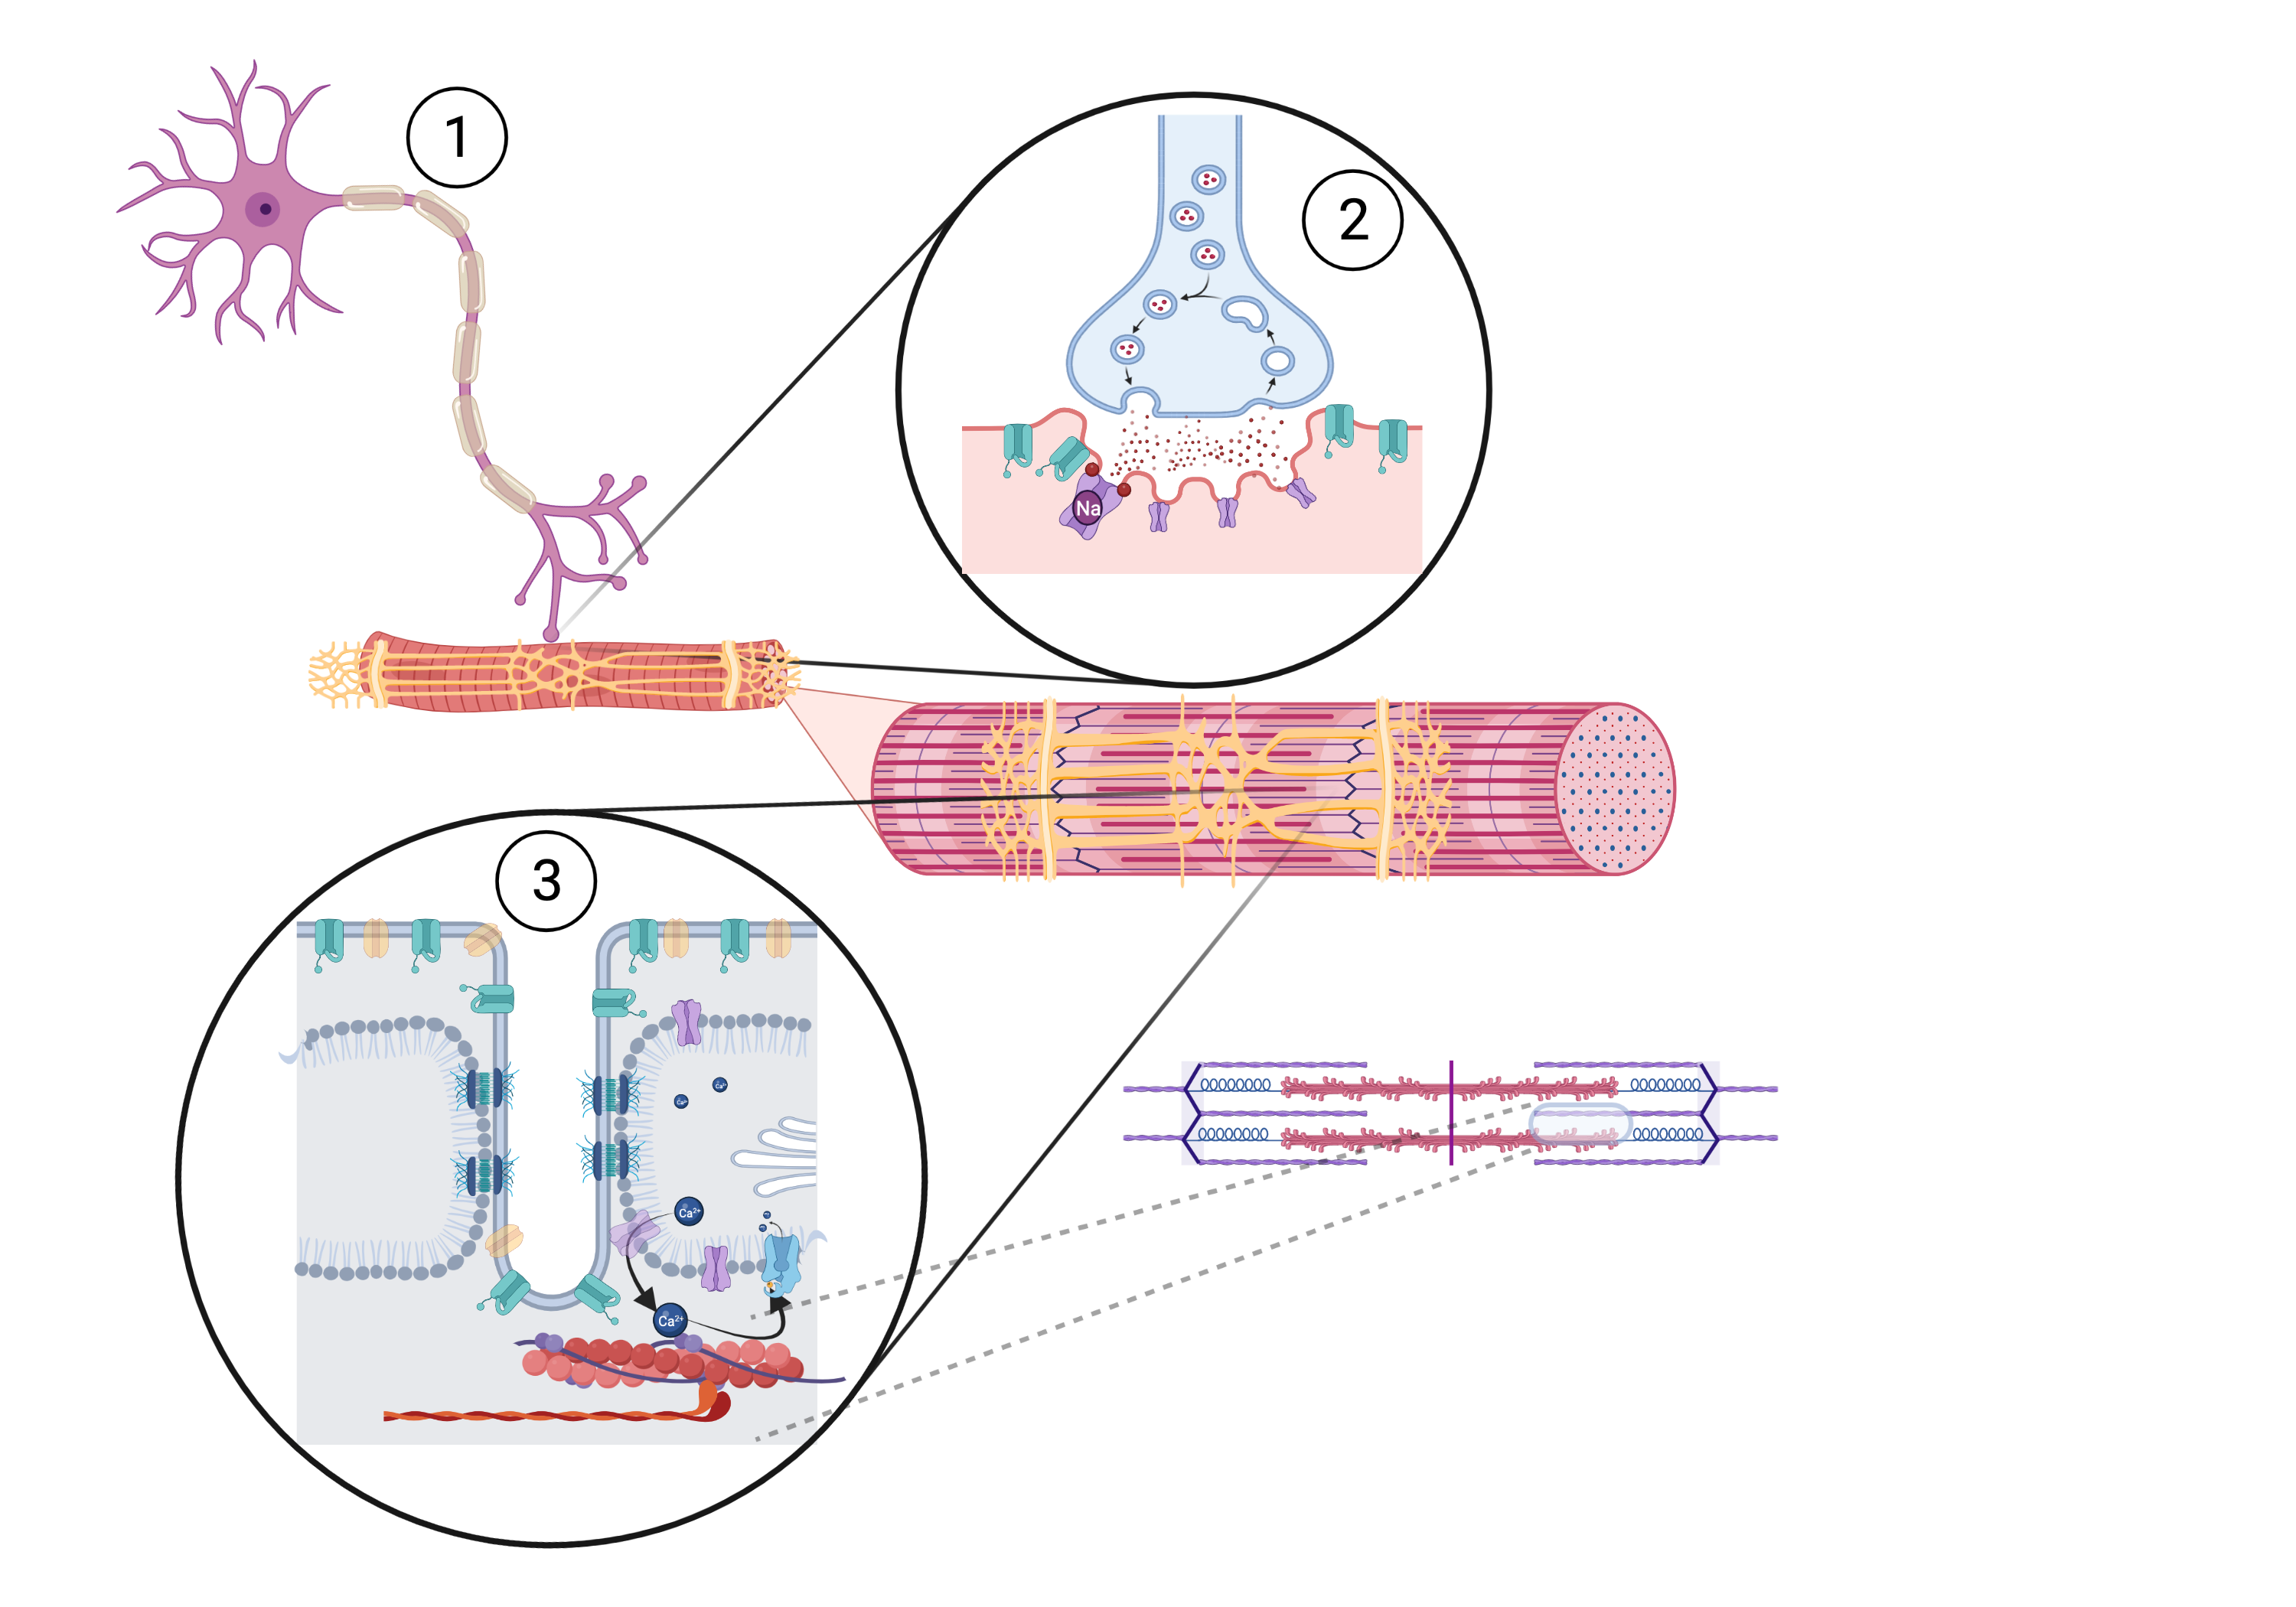
\includegraphics[width=1\linewidth]{./figure/excitation_overview.png}
    \caption{Overview of excitation from the $\alpha$ motor neuron to crossbridge activation \footnotesize{Created with BioRender.com}}
    \label{fig:excitation_overview}
\end{figure}

\subsection{Step 1 - The $\alpha$-Motor Neuron}
Excitation of an $\alpha$-motor neuron is regulated by the central nervous system and occurs at the membrane of its dendrites in the spinal cord. A wave of excitation travels along the axon to its terminal branches at neuromuscular junctions (NMJs) by sequential excitation facilitated by voltage gated ion channels. Each muscle fiber has one NMJ and receives one axon terminal. However, each $\alpha$-motor neuron has a variable number of terminal branches (Chapter \ref{chp:regulation}).  Excitation travels from the spinal cord to the NMJ by means of saltatory conduction which allows excitation to take big steps as it travels along the axon membrane. Saltatory conduction increases the nerve conduction velocity and is made possible by the myelin sheathes (Figure \ref{fig:Motoneuron}). The membrane is exposed along the axon at nodes of Ranvier. Excitation travels by jumping from one node of Ranvier to the next.\footnotemark\footnotetext{The implications of the myelin sheath on nerve conduction velocity is detailed in Chapter \ref{chp:regulation} as an important consideration for muscle tension regulation.} 

\begin{figure}[!ht]
    \centering
    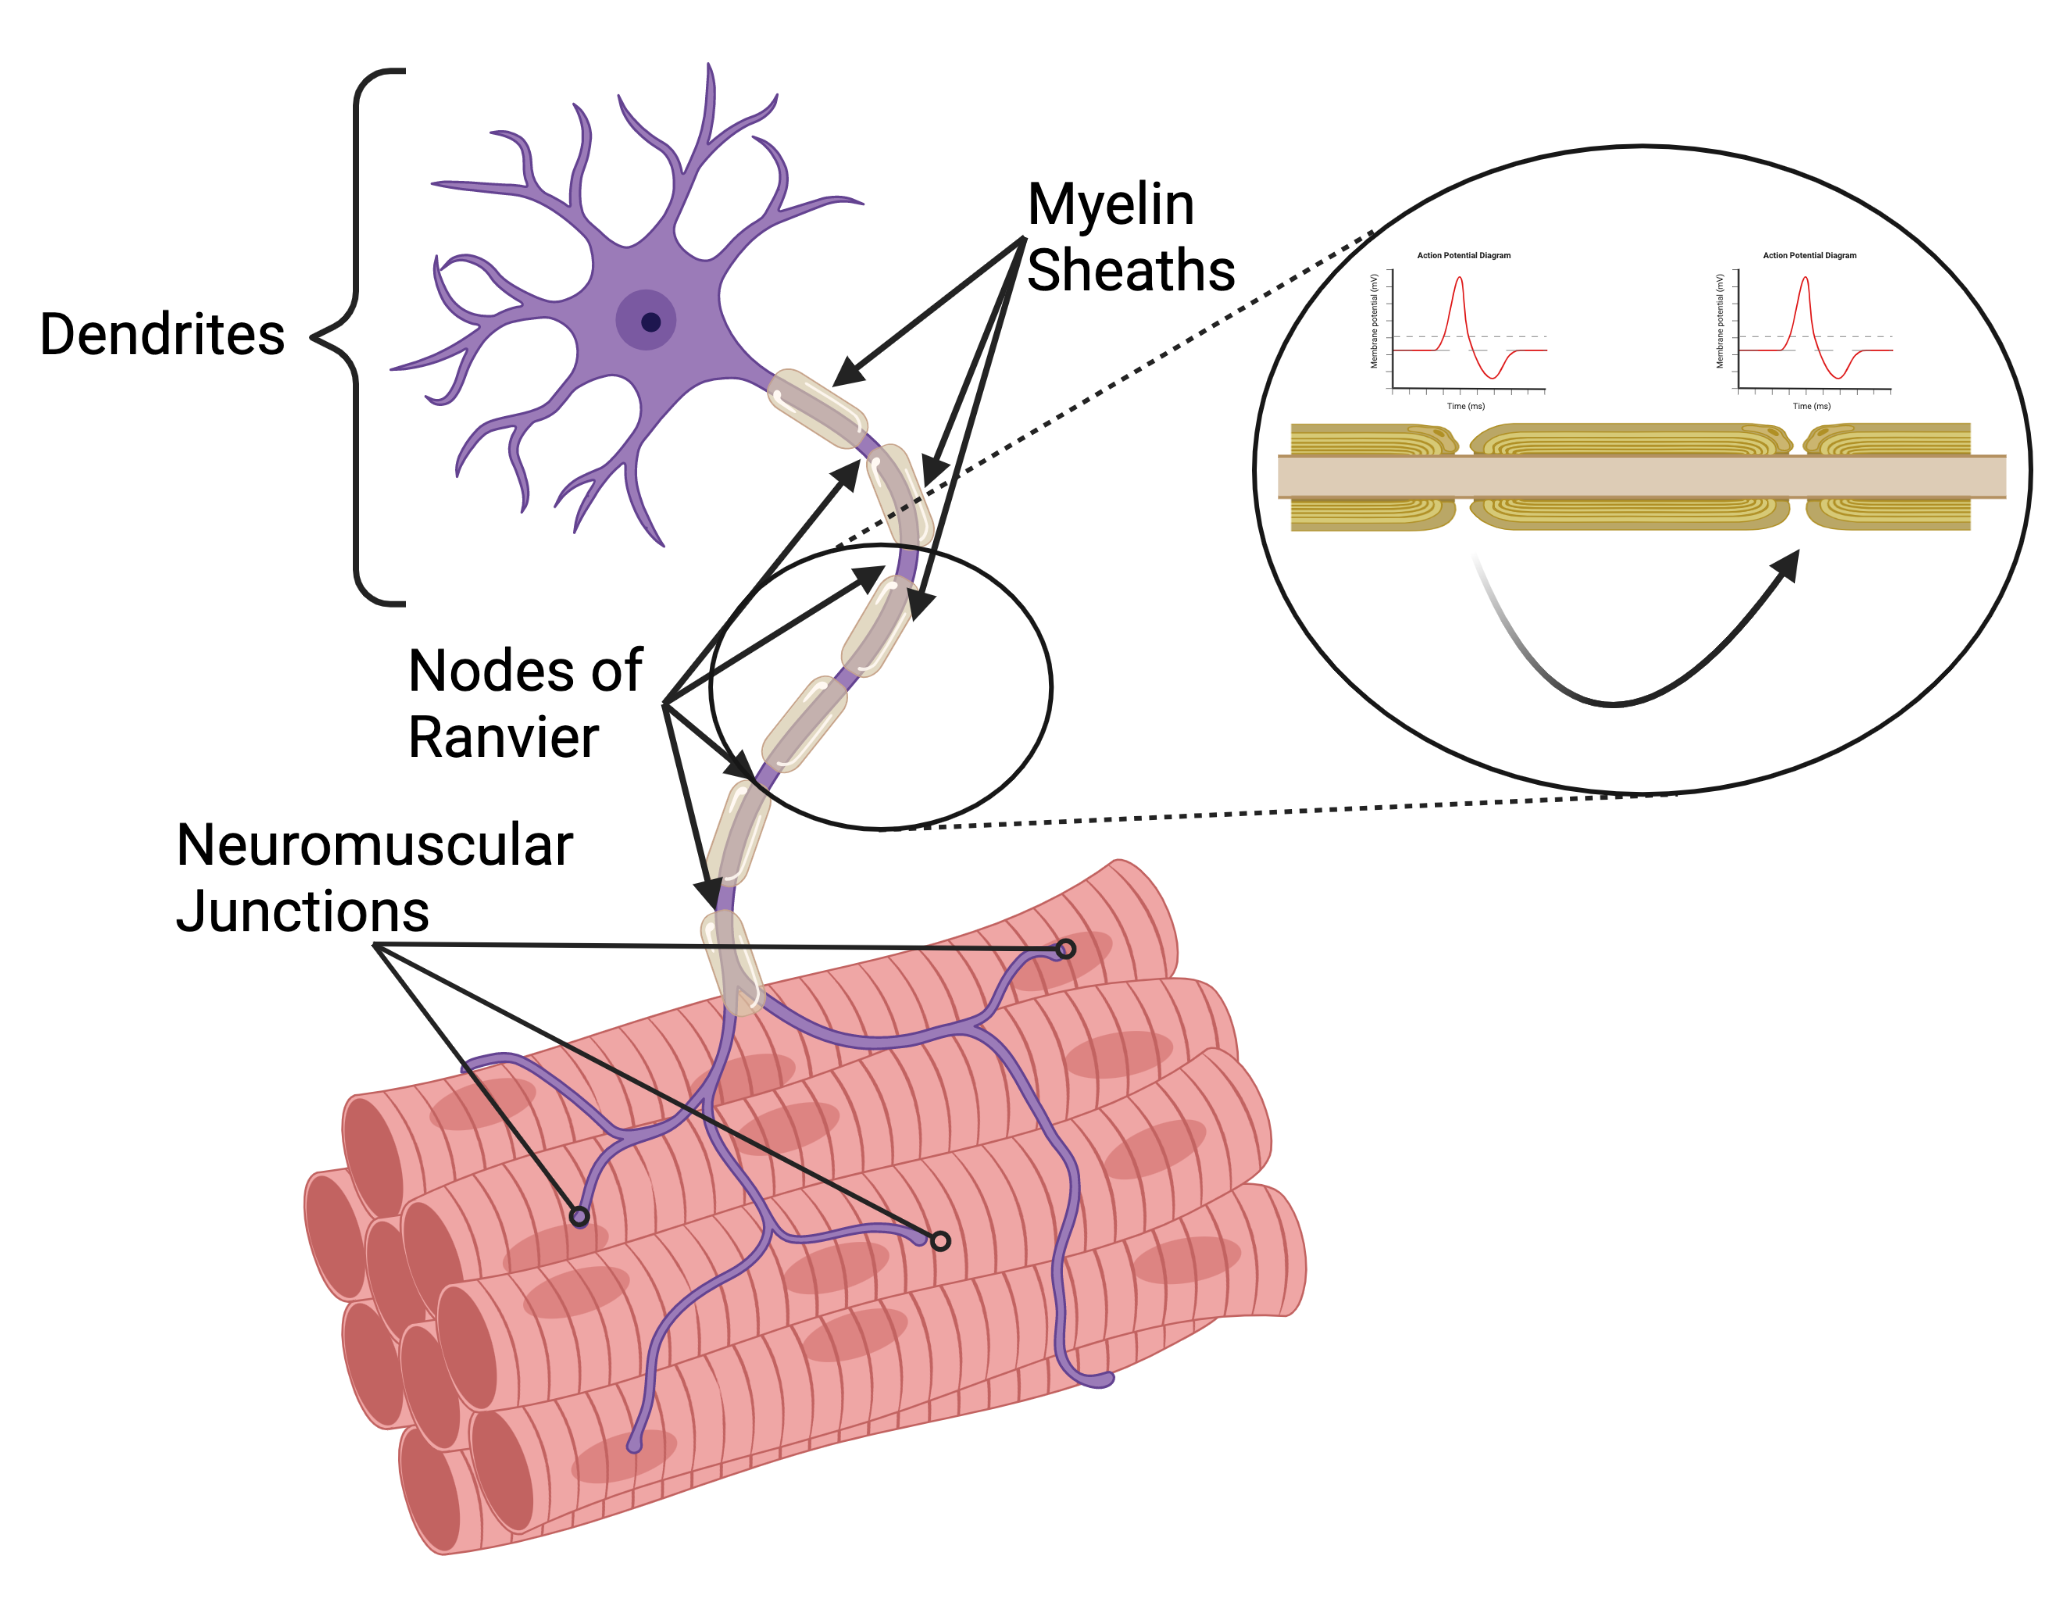
\includegraphics[width=1\linewidth]{./figure/Motoneuron.png}
    \caption{$\alpha$-motor neuron terminating at several muscle fiber motor end plates \footnotesize{Created with BioRender.com}}
    \label{fig:Motoneuron}
\end{figure}

\subsection{Step 2 - Neuromuscular Junction - Motor End Plate - Sarcolemma Excitation}

Membrane excitation at the axon terminal releases the neurotransmitter acetylcholine (ACh) due to the action of voltage gated $Ca^{2+}$ channels signaling exocytosis of vesicles filled with ACh. ACh crosses the NMJ synapse (Figure \ref{fig:NMJ} and excites the motor end plate by binding to receptors and opening ligand gated $Na^+$ ion channels. For tight regulation of muscle activation at the NMJ, ACh is quickly broken down by cholinesterase (an enzyme synthesized by the muscle fiber that hydrolyzes ACh) and free choline molecules are transported into the axon terminal (endocytosis) to be resynthesized. However, when high concentrations of ACh accumulate at the NMJ (due to a high frequency of axon excitations) there are two processes that can result in more rapid excitation of the motor end plate.\footnotemark\footnotetext{"More rapid" means generating the motor end plate excitation faster to allow for the higher frequency of excitation, not that the motor end plate ends up having a higher frequency of excitation than the axon. Such decoupling of $\alpha$-motor axon excitation and motor end plate excitation would create additional challenges to motor control.} Temporal summation of receptors refers to repeated stimulation of one receptor by ACh; and spatial summation of receptors refers to stimulation of a larger number of motor end plate receptors. Frequency summation is limited by the amount of ACh, which is influenced by the release of ACh from the axon terminal and the breakdown of ACh in the NMJ. Spatial summation is also limited by the amount of ACh, but it is also limited by the number of receptors on the motor end plate, and is therefore adaptable over time through cellular regulatory processes (making more receptors (up regulating), or reducing the number of receptors (down regulating).

% axon terminal voltage gated Ca+ channels are inhibited by high magnesium ($Mg^{2+}$) concentrations. - not sure why I had that random fact in the middle of the paragraph - but I'm not ready to get rid of it yet because if I can expand on it and make come clinical connection it could be worthwhile.

\begin{figure}[!ht]
    \centering
    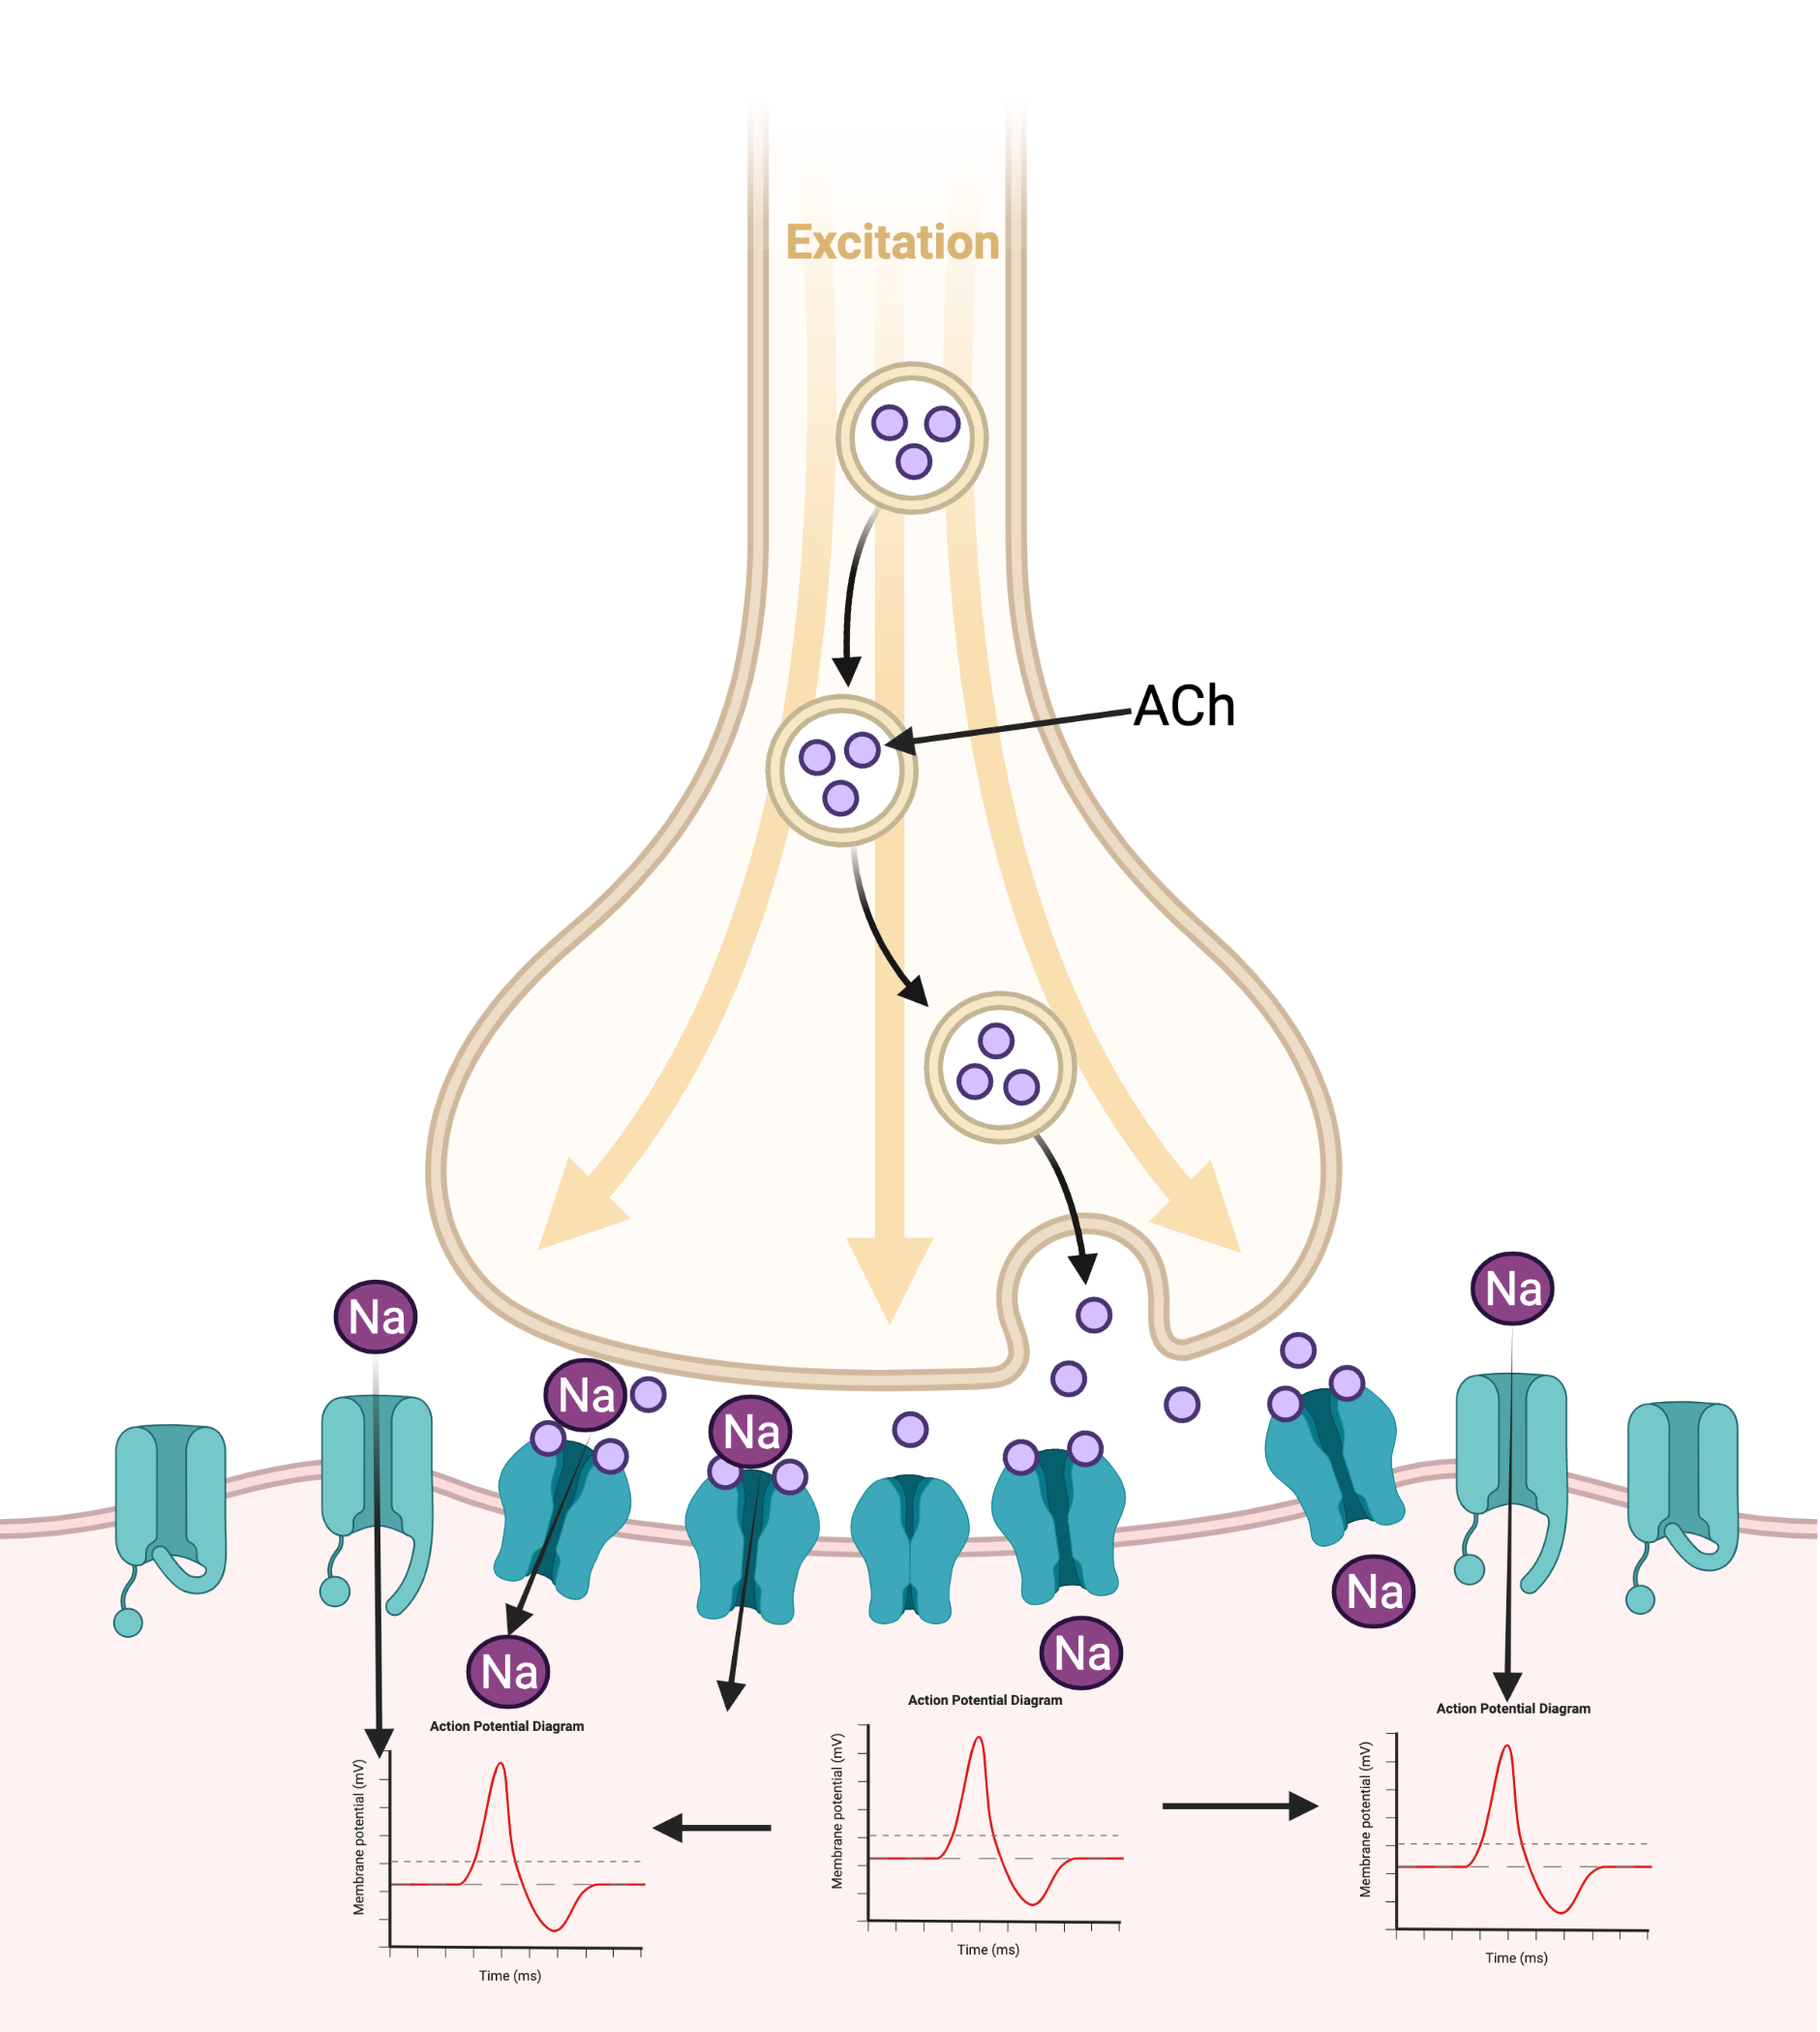
\includegraphics[width=1\linewidth]{./figure/NMJ.png}
    \caption{NMJ Excitation of the Motor End Plate \footnotesize{Created with BioRender.com}}
    \label{fig:NMJ}
\end{figure}

Excitation of the motor end plate spreads to the sarcolemma due to the opening of voltage gated ion channels on the sarcolemma. Sarcolemma excitation creates a wave similar to that in the axon (but without myelin) that spreads due to opening of voltage gated ion channels. The sarcolemma surrounds the fiber and penetrates the fiber and circles myofibrils through the intricate T-tubule system. T-tubules that encircle myofibrils form a triad with a SR on each side (See Figure \ref{fig:T-tubule}).

% Import the T-Tubule - SR triad image - CC from wikipedia

\begin{figure}[!ht]
    \centering
    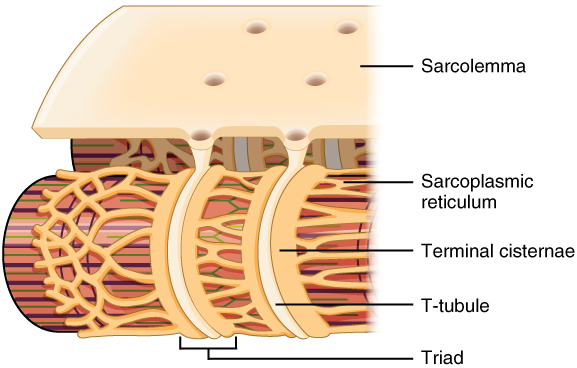
\includegraphics[width=1\linewidth]{./figure/T-tubule.jpg}
    \caption{T-Tubule Encircling a Myofibril \& Forming a Triad with Sarcoplasmic Reticulum  \footnotesize{(OpenStax, CC BY 4.0, \href{https://creativecommons.org/licenses/by/4.0}{via Wikimedia Commons})}}
    \label{fig:T-tubule}
\end{figure}

\subsection{Step 3 - Excitation - Activation Coupling (EAC)}
Excitation of the T-tubules excites the sarcoplasmic reticulum (SR). There are unique junctions between T tubules and the SR mediated by $Ca^{2+}$ channels. One acts as a voltage sensor in the T tubules, and a second acts as $Ca^{2+}$ release channels in the SR.\footnotemark{}\footnotetext{The position of these two calcium channels differ between skeletal and cardiac muscle, which correlates with the functional differences in the control of contraction between these two types of muscle.} The functional implication of this unique T-tubule - SR junction is that excitation of the T-tubule quickly results in a combined excitation of the SR along with the release of $Ca^{2+}$ into the sarcoplasm\footnotemark\footnotetext{Sarcoplasm is the muscle fiber equivalent of the cytoplasm, the intracellular region that is in the cell but outside of any organelles (such as the SR, nucleus, mitochondria).} in close proximity of troponin binding sites for crossbridge activation (Figure \ref{fig:SR}).

\begin{figure}[!ht]
    \centering
    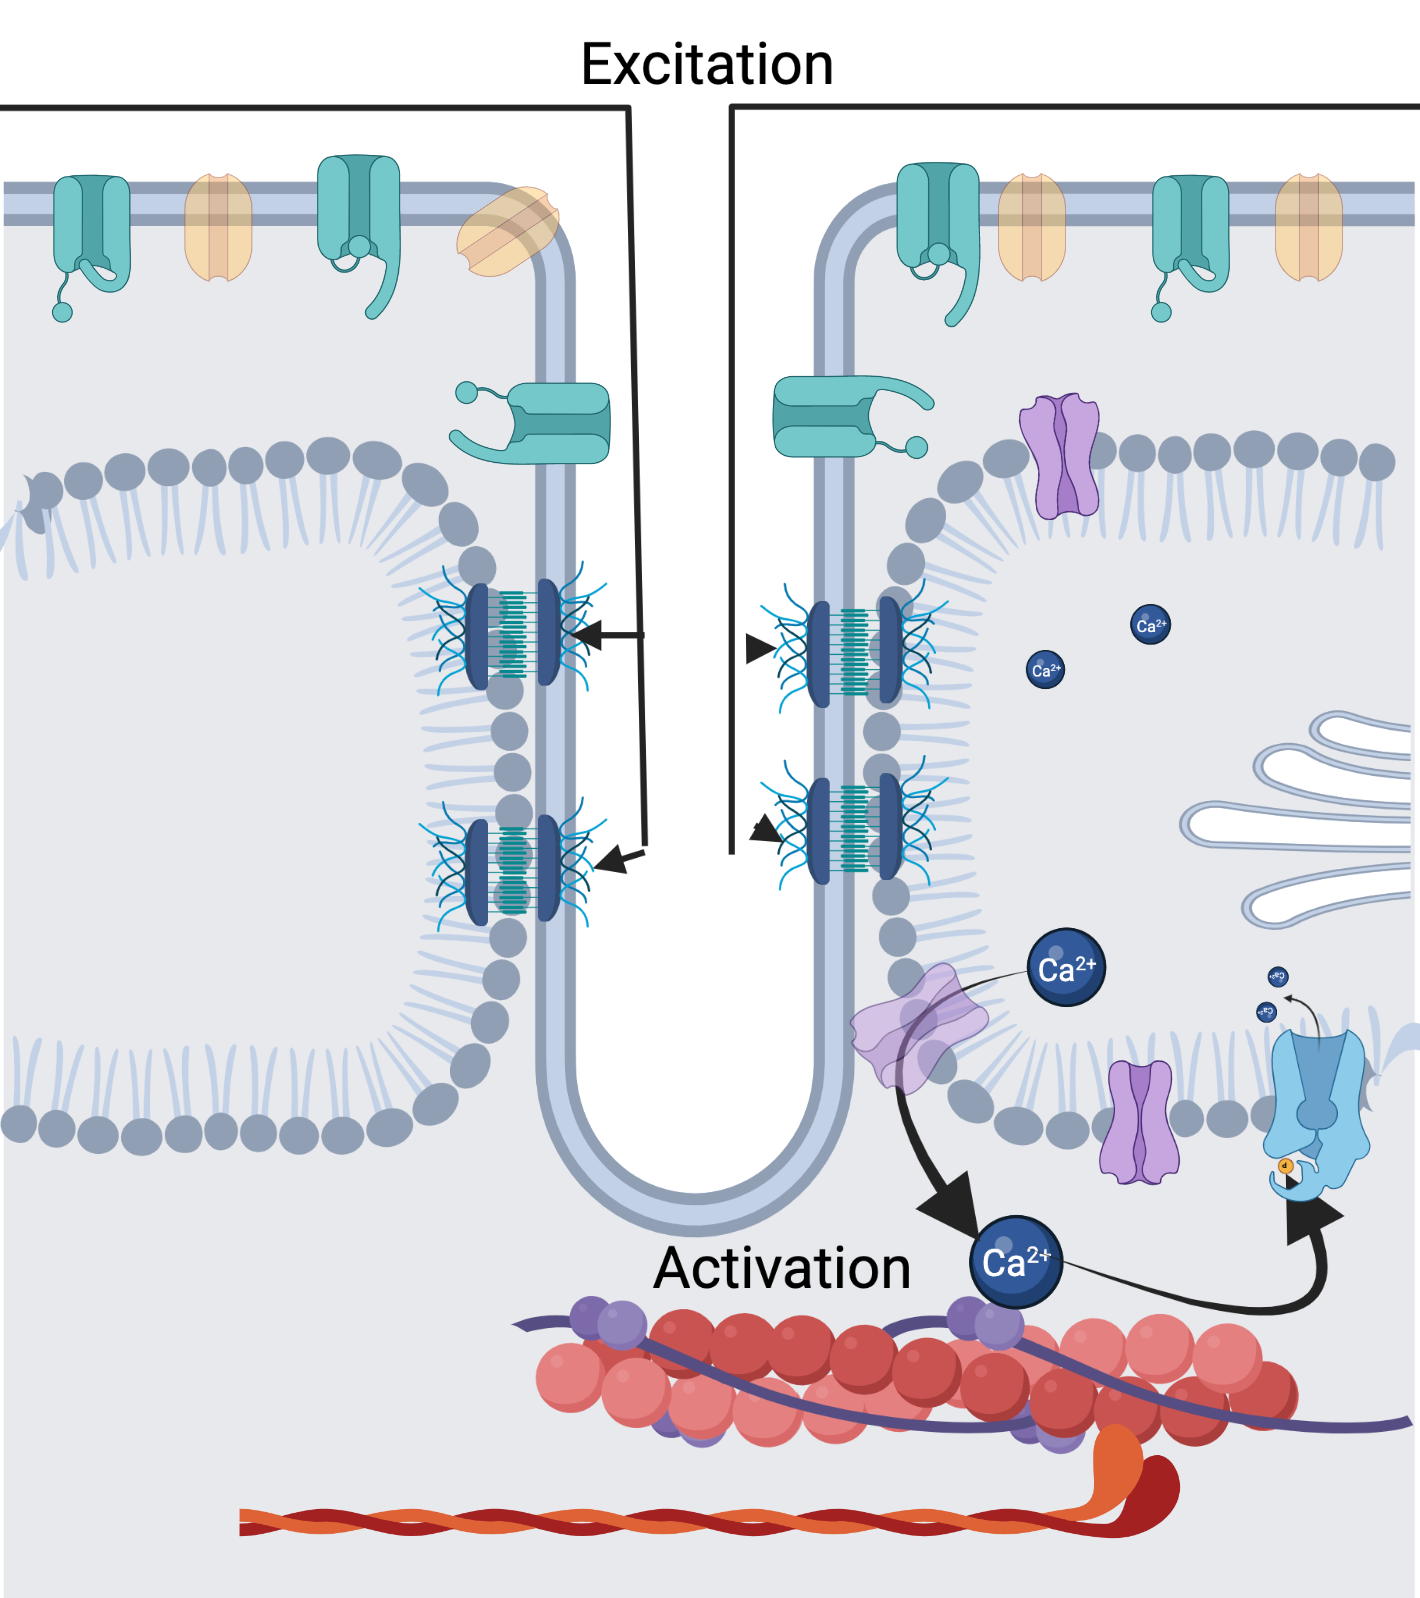
\includegraphics[width=1\linewidth]{./figure/SR.png}
    \caption{Sarcoplasmic Reticulum as the site of Excitation-Activation Coupling \footnotesize{Created with BioRender.com}}
    \label{fig:SR}
\end{figure}

\paragraph{Excitation \& EAC Latency}

Figure \ref{fig:eac-latency} represents each major phase of excitation and EAC from the $\alpha$-motor neuron to development of a twitch. The latency period time scale is in milliseconds (ms, 1/1000 of a second). The latency period of each excitation and EAC forms an upper boundary on the number of possible twitches per second. However, this boundary is determined by the latency of the excitation portion of Figure \ref{fig:eac-latency} which amounts to a few milliseconds. The fact that the twitch lasts for an estimated 100 ms means that excitation (a few milliseconds) can occur at a frequency that results in twitch summation since each twitch takes about 100 milliseconds they can sum together to produce tetany.

\begin{figure}[!ht]
    \centering
    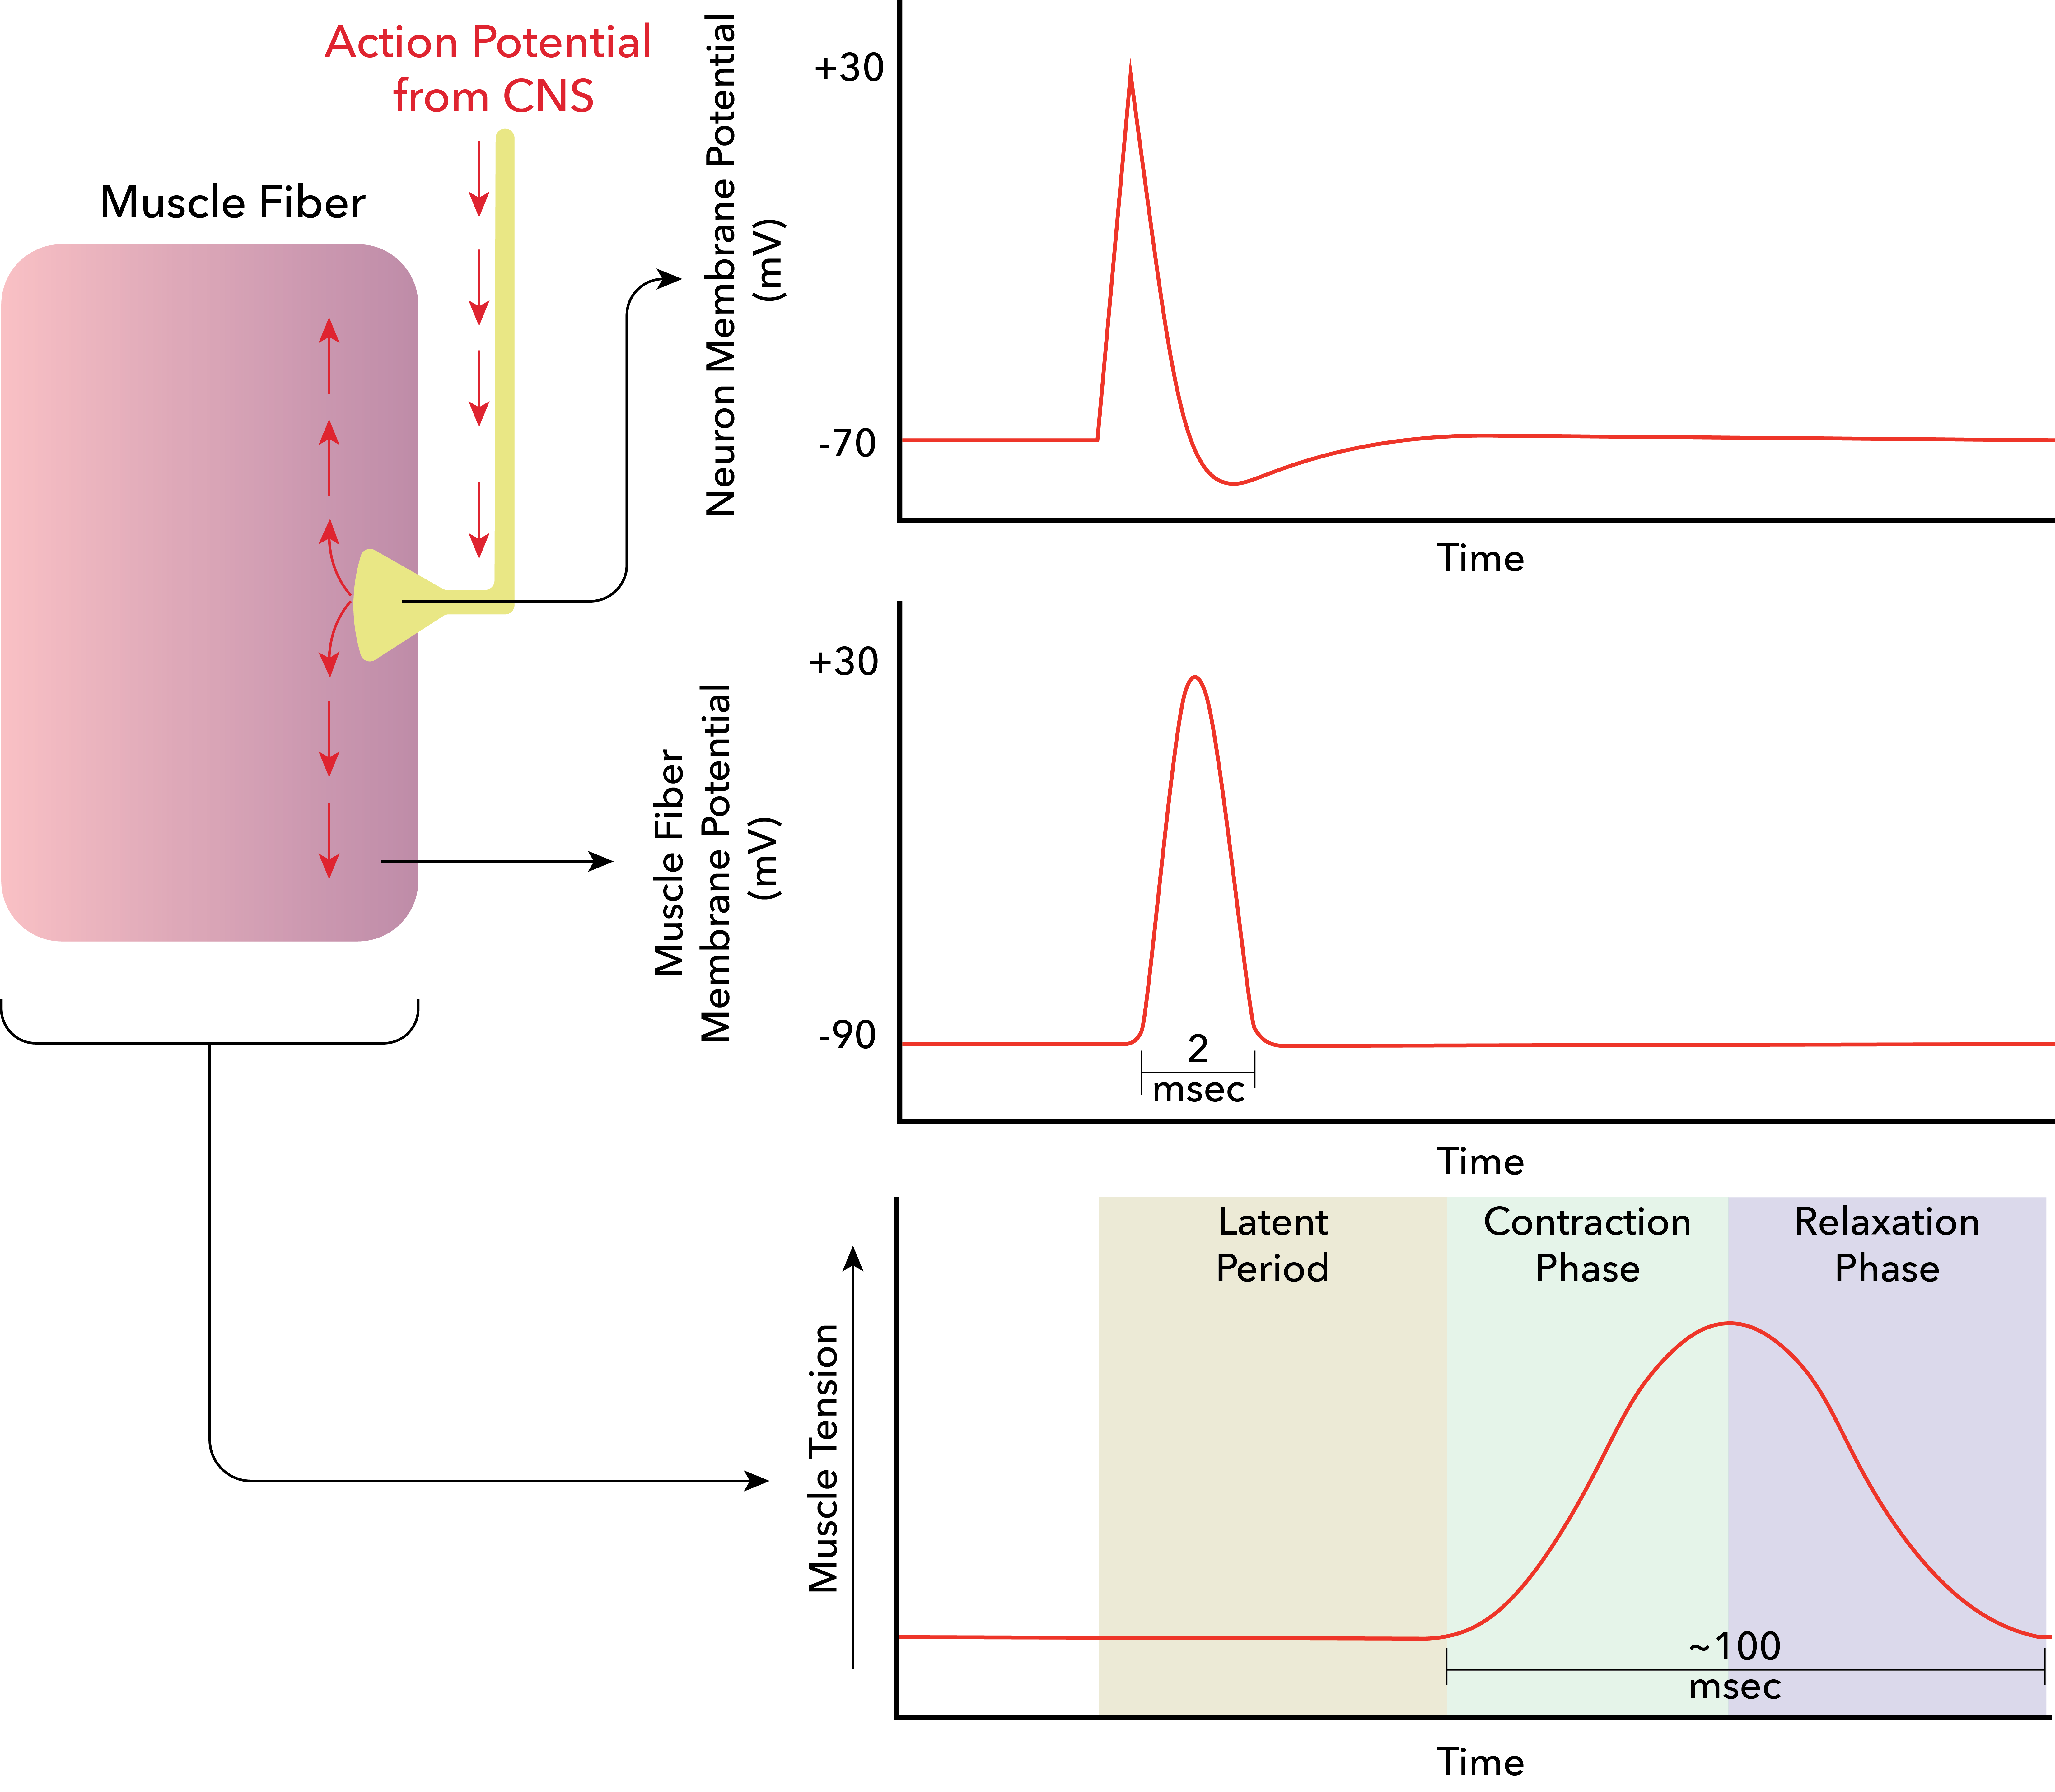
\includegraphics[width=1\linewidth]{./figure/eac-latency.png}
    \caption{EAC Latency \footnotesize{(Wikimedia Commons, CC BY 4.0, \href{https://commons.wikimedia.org/wiki/File:The_latent_period_between_the_muscle_action_potential_and_contraction.png}{EAC-Latency})}}
    \label{fig:eac-latency}
\end{figure}

\subsubsection{Twitch to Tetany}
Each excitation activates enough crossbridges to produce a twitch. A twitch is the fundamental unit of active tension. However, a single twitch of active tension is not enough tension when the goal of tension is some sort of voluntary movement or stability. The rise and rate of a twitch depends on the amount and spread of $Ca^{2+}$ released, the available troponin sites, the available crossbridges to activate as well as the amount of elasticity in the series. One mechanism of muscle fatigue is a reduction in the release of $Ca^{2+}$ from the SR. The rate of $Ca^{2+}$ release from the SR can be increased in experimental preparations with caffeine. Low concentrations of caffeine bind to the voltage gated $Ca^{2+}$ channels at the junction of the T-tubule SR and increase $Ca^{2+}$ release during otherwise normal activation. However, high concentrations result in contracture without the need for the normal excitation signal. 

%A twitch can be an experimentally manipulated event. An electrical stimulus is provided to a muscle which results in either, or a combination of, $\alpha$-motor neuron excitation and sarcolemma excitation that excites the SR and activates enough crossbridges to produces enough active tension to produce a measurable force. A twitch can also be initiated by isolated (single) excitation of an $\alpha$-motor neuron, or isolated excitation of an $\alpha$-motor neuron or sarcolemma. 


\paragraph{Tetany}
Repeated excitation results in repeated activation and therefore continued crossbridge activation and repeated twitches (Figure \ref{fig:tetany}). Successive twitches create tension summation and is called tetany. When the force of active tension is measured, such as during a muscle test, it is the result of many muscle fibers being in tetany. The use of twitch frequency to create tetany and regulate active tension is detailed in Chapter \ref{chp:regulation}. 

\begin{figure}[!ht]
    \centering
    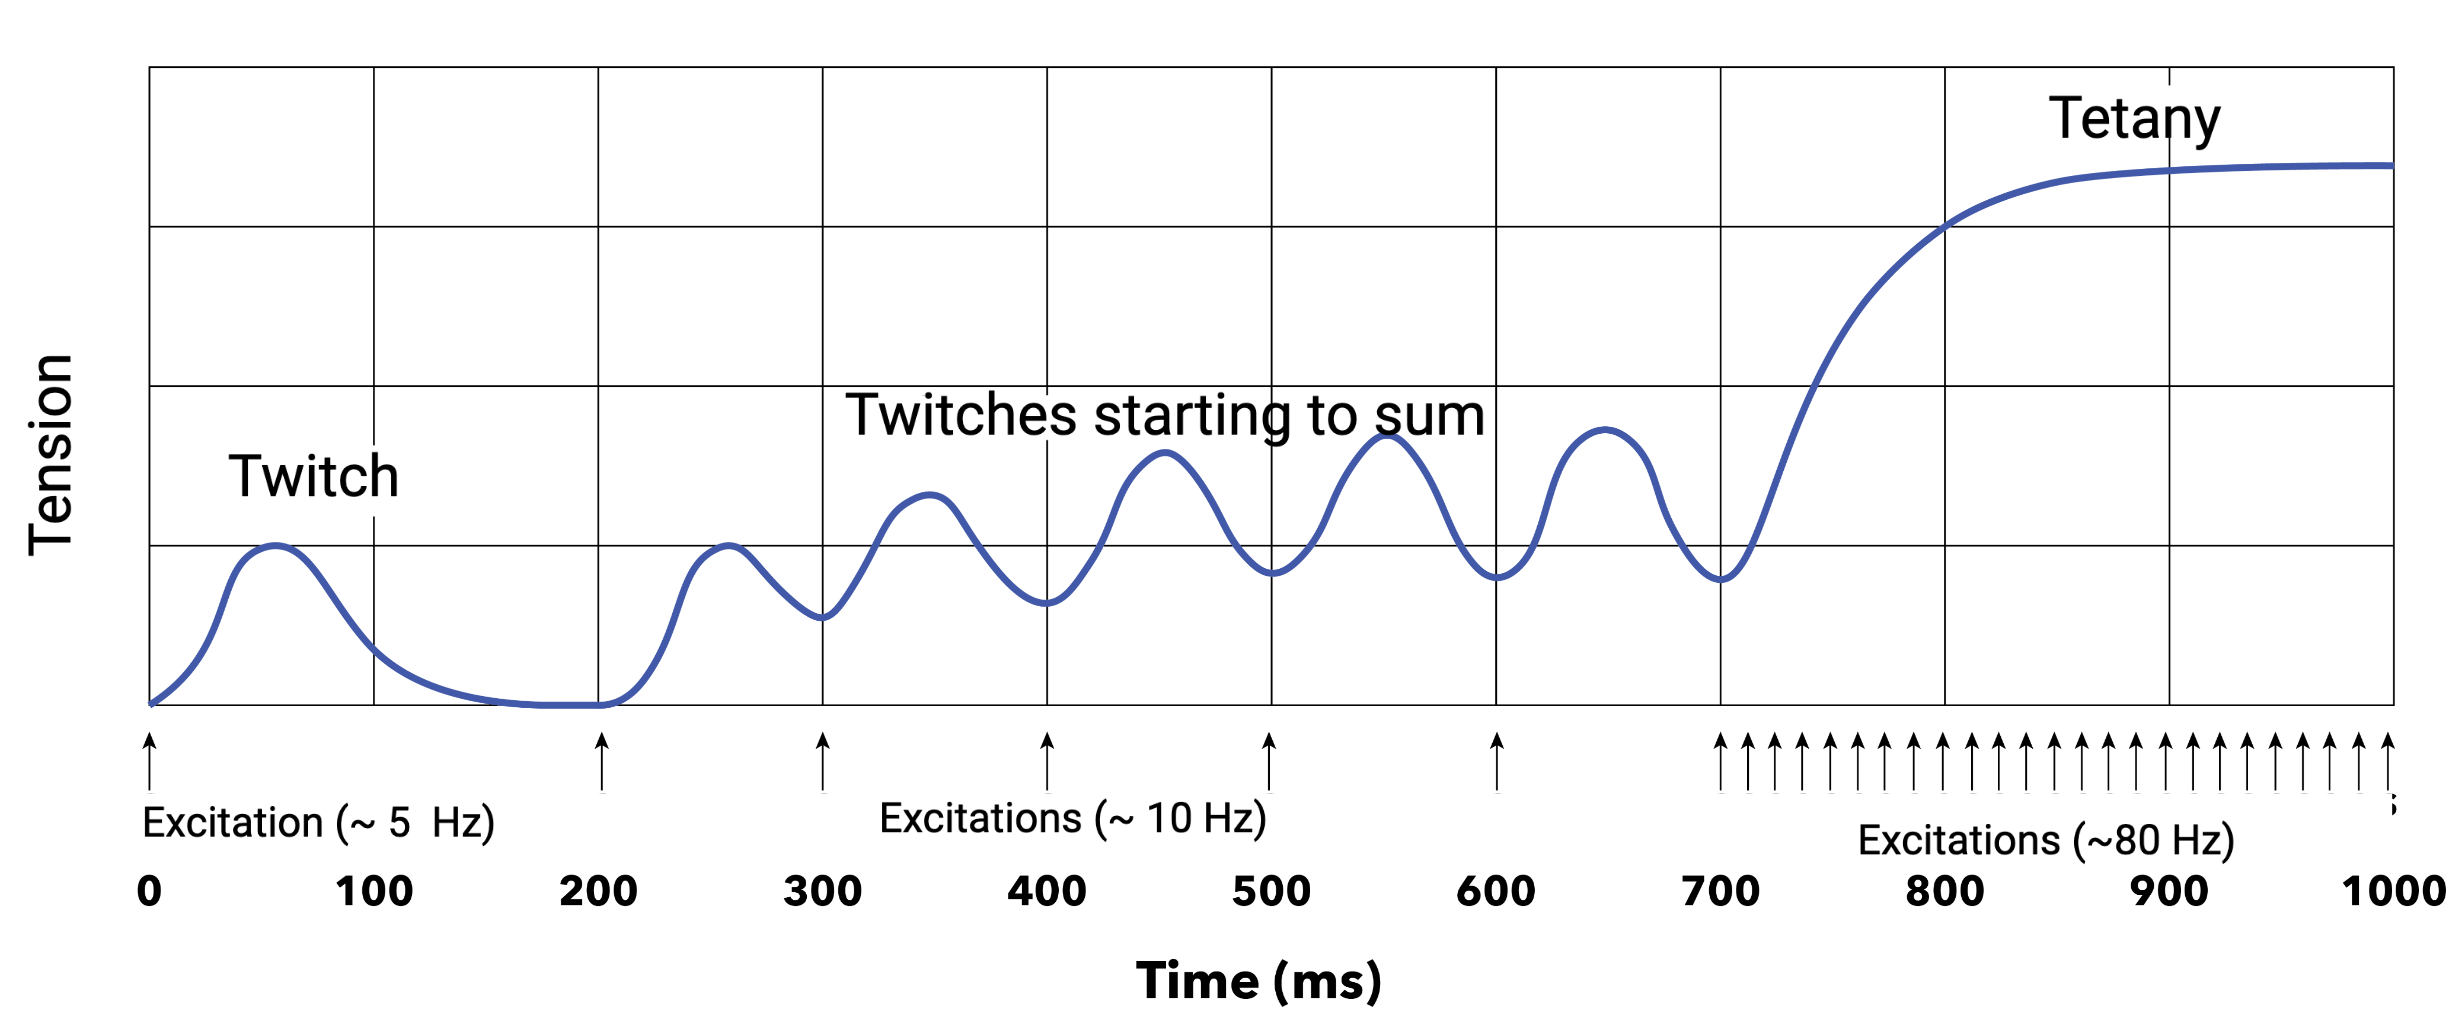
\includegraphics[width=1\linewidth]{./figure/tetany.png}
    \caption{EAC Latency \footnotesize{Modified with BioRender.com from \href{https://commons.wikimedia.org/wiki/File:Twitch_vs_unfused_tetanus_vs_fused_tetanus.png}{Wikimedia Commons, CC BY 4.0})}}
    \label{fig:tetany}
\end{figure}

\subsubsection{Removal of Ca from Sarcoplasm}
Removal of $Ca^{2+}$ from the sarcoplasm requires active transport with $Ca^{2+}$ ATPase. This pump is dependent on $Mg^{2+}$ and moves 2 $Ca^{2+}$ into the SR while moving one $H^+$ out at the cost of 1 ATP. Sarcoplasm levels of $Ca^{2+}$ can quickly return to resting levels which is necessary for rapid muscle relaxation and therefore muscle tension regulation and coordination. Situations that result in a delay in the removal of $Ca^{2+}$ from the sarcoplasm can delay muscle relaxation producing extra twitches or spasms (involuntary tetany). Since $Ca^{2+}$ ATPase is dependent on $Mg^{2+}$, a deficiency in $Mg^{2+}$ can create such a situation.

% Start getting read to transition to a more detailed description of excitation

\subsection{Return to Resting (Non excitation) State - RMP}
The process of returning to the resting state (RMP) is not explicitly discussed in the above sequence of membrane excitation events. It is implied, or taken for granted, once we started discussing the excitation of a twitch to the excitation of tetany (the summation of many twitches). Excitation of tetany requires that the axon, axon terminal, motor end plate, sarcolemma and T-tubule return to a resting (non excited) state. Notice, there is no excitation summation, only twitch summation.

\paragraph{}
Excitation occurs quickly because the resting state includes potential energy for excitation. The RMP is a polarized membrane with large ion concentration gradients (just waiting to run downhill with their gradients). This potential energy comes at a cost of spending energy (ATP) to pump ions against a concentration gradient. The RMP enables rapid excitation because ions are waiting with potential energy due to their concentration gradient to move quickly across the membrane (depolarize). 

\paragraph{}
The RMP also enables rapid return to the resting state with potential energy. The movement of $K^+$ and $Cl^-$ ions with their concentration gradient can quickly end excitation enabling the membrane to be quickly returned to RMP for another excitation. However the long term stability of the RMP relies on processes that depend on ion pumps to sustain concentration gradients for a lifetime.\footnotemark\footnotetext{Brain and heart death are situations where the cells of the brain and heart no longer return to the resting state, they no longer repolarize to the RMP, and therefore they can no longer undergo excitation.}
A deeper understanding of excitation and return to RMP, and clinical connections, requires a molecular and cellular understanding of excitable membranes.

% Second lap on excitation - not every step, and more detailed

\section{Excitable Membranes}

An excitable membrane is polarized in its resting state, which is the resting membrane potential (RMP). An excitable membrane can be excited (experience excitation) when the membrane loses its polarity, which is called depolarization. Depolarization is what occurs during an action potential (AP). What makes the membrane able to be depolarized is the fact that it is polarized. What makes the membrane capable of an AP is the fact that it has a RMP. Please excuse the repetition. But since these terms are all used rather interchangeably it is important that the reader develop a familiarity with the concepts with the exchange of language. The use of the various terms in the book is simply a reflection of the unfortunate situation of various terms being used across fields, papers, and other books.

For emphasis, a membrane cannot depolarize unless it is polarized. To understand muscle excitation and regulation\footnotemark\footnotetext{muscles are regulated through variations in excitation} requires understanding how the RMP is established, how the RMP depolarizes with an action potential (AP), and how the AP propagates (spreads as a wave of excitation). Understanding these concepts also opens the door to understanding several additional topics in clinical physiology. 



% Old but not ready to delete so commented out....
%Signal transmission that results in cellular events (including along the membrane) it is called signal transduction. The action potential signal transduction that occurs along the surface of a nerve and muscle membrane is facilitated by the presence of voltage gated channels embedded in the membrane. Signal transduction from a membrane to another membrane is facilitated by ligand gated channels at specific places in membrane. The detailed physiology of excitable membranes such as establishing and maintaining a resting membrane potential, and mechanisms that result in action potentials are important details covered later in the chapter. 
%------------------
\subsection{Resting Membrane Potential}

The RMP requires several particular characteristics and actions of the cell membrane, and in the case of a muscle fiber, the sarcolemma.

\subsubsection{Sarcolemma}

The sarcolemma is a semipermeable phospholipid bilayer membrane that forms a boundary for the muscle fiber. Semi-permeability arises in part because of the bilayer being hydrophobic (detracts water) and the inside of the membrane being hydrophilic (attracts water) which limits what can freely diffuse through the membrane (for example oxygen and carbon dioxide can freely pass through the the sarcolemma). A large part of the semi-permeability arises from the particular transport proteins within the membrane for selective forms of active, facilitated and passive transport.\footnotemark\footnotetext{As a refresher, active transport utilizes protein machines that require ATP and move very specific molecules, typically, against a concentration gradient. Facilitated transport utilizes protein machines to move very specific molecules across the membrane without the need for ATP. Facilitated transport requires a concentration gradient for at least one molecule, but can be coupled with another molecule that moves against a concentration gradient. Meaning, facilitated transport can utilize the potential energy of one molecule to provide the energy needed to move another molecule against a gradient. Passive transport occurs due to a concentration gradients (such as simple or channel guided diffusion).} The membrane separates the intracellular from the extra cellular space. Through selective transport the membrane establishes the conditions for cellular activities within the cell and thus influences (but does not completely establish) conditions outside the cell. Sarcolemma (all cell membranes) are dynamic structures that adapt in response to the intracellular and extra cellular conditions to meet the needs of the cell.

Components of the sarcolemma that are discussed below and that play an important role for establishing the resting membrane potential as well as the action potential are depicted in Figure \ref{fig:cell_membrane}. 

\begin{figure}[!ht]
    \centering
    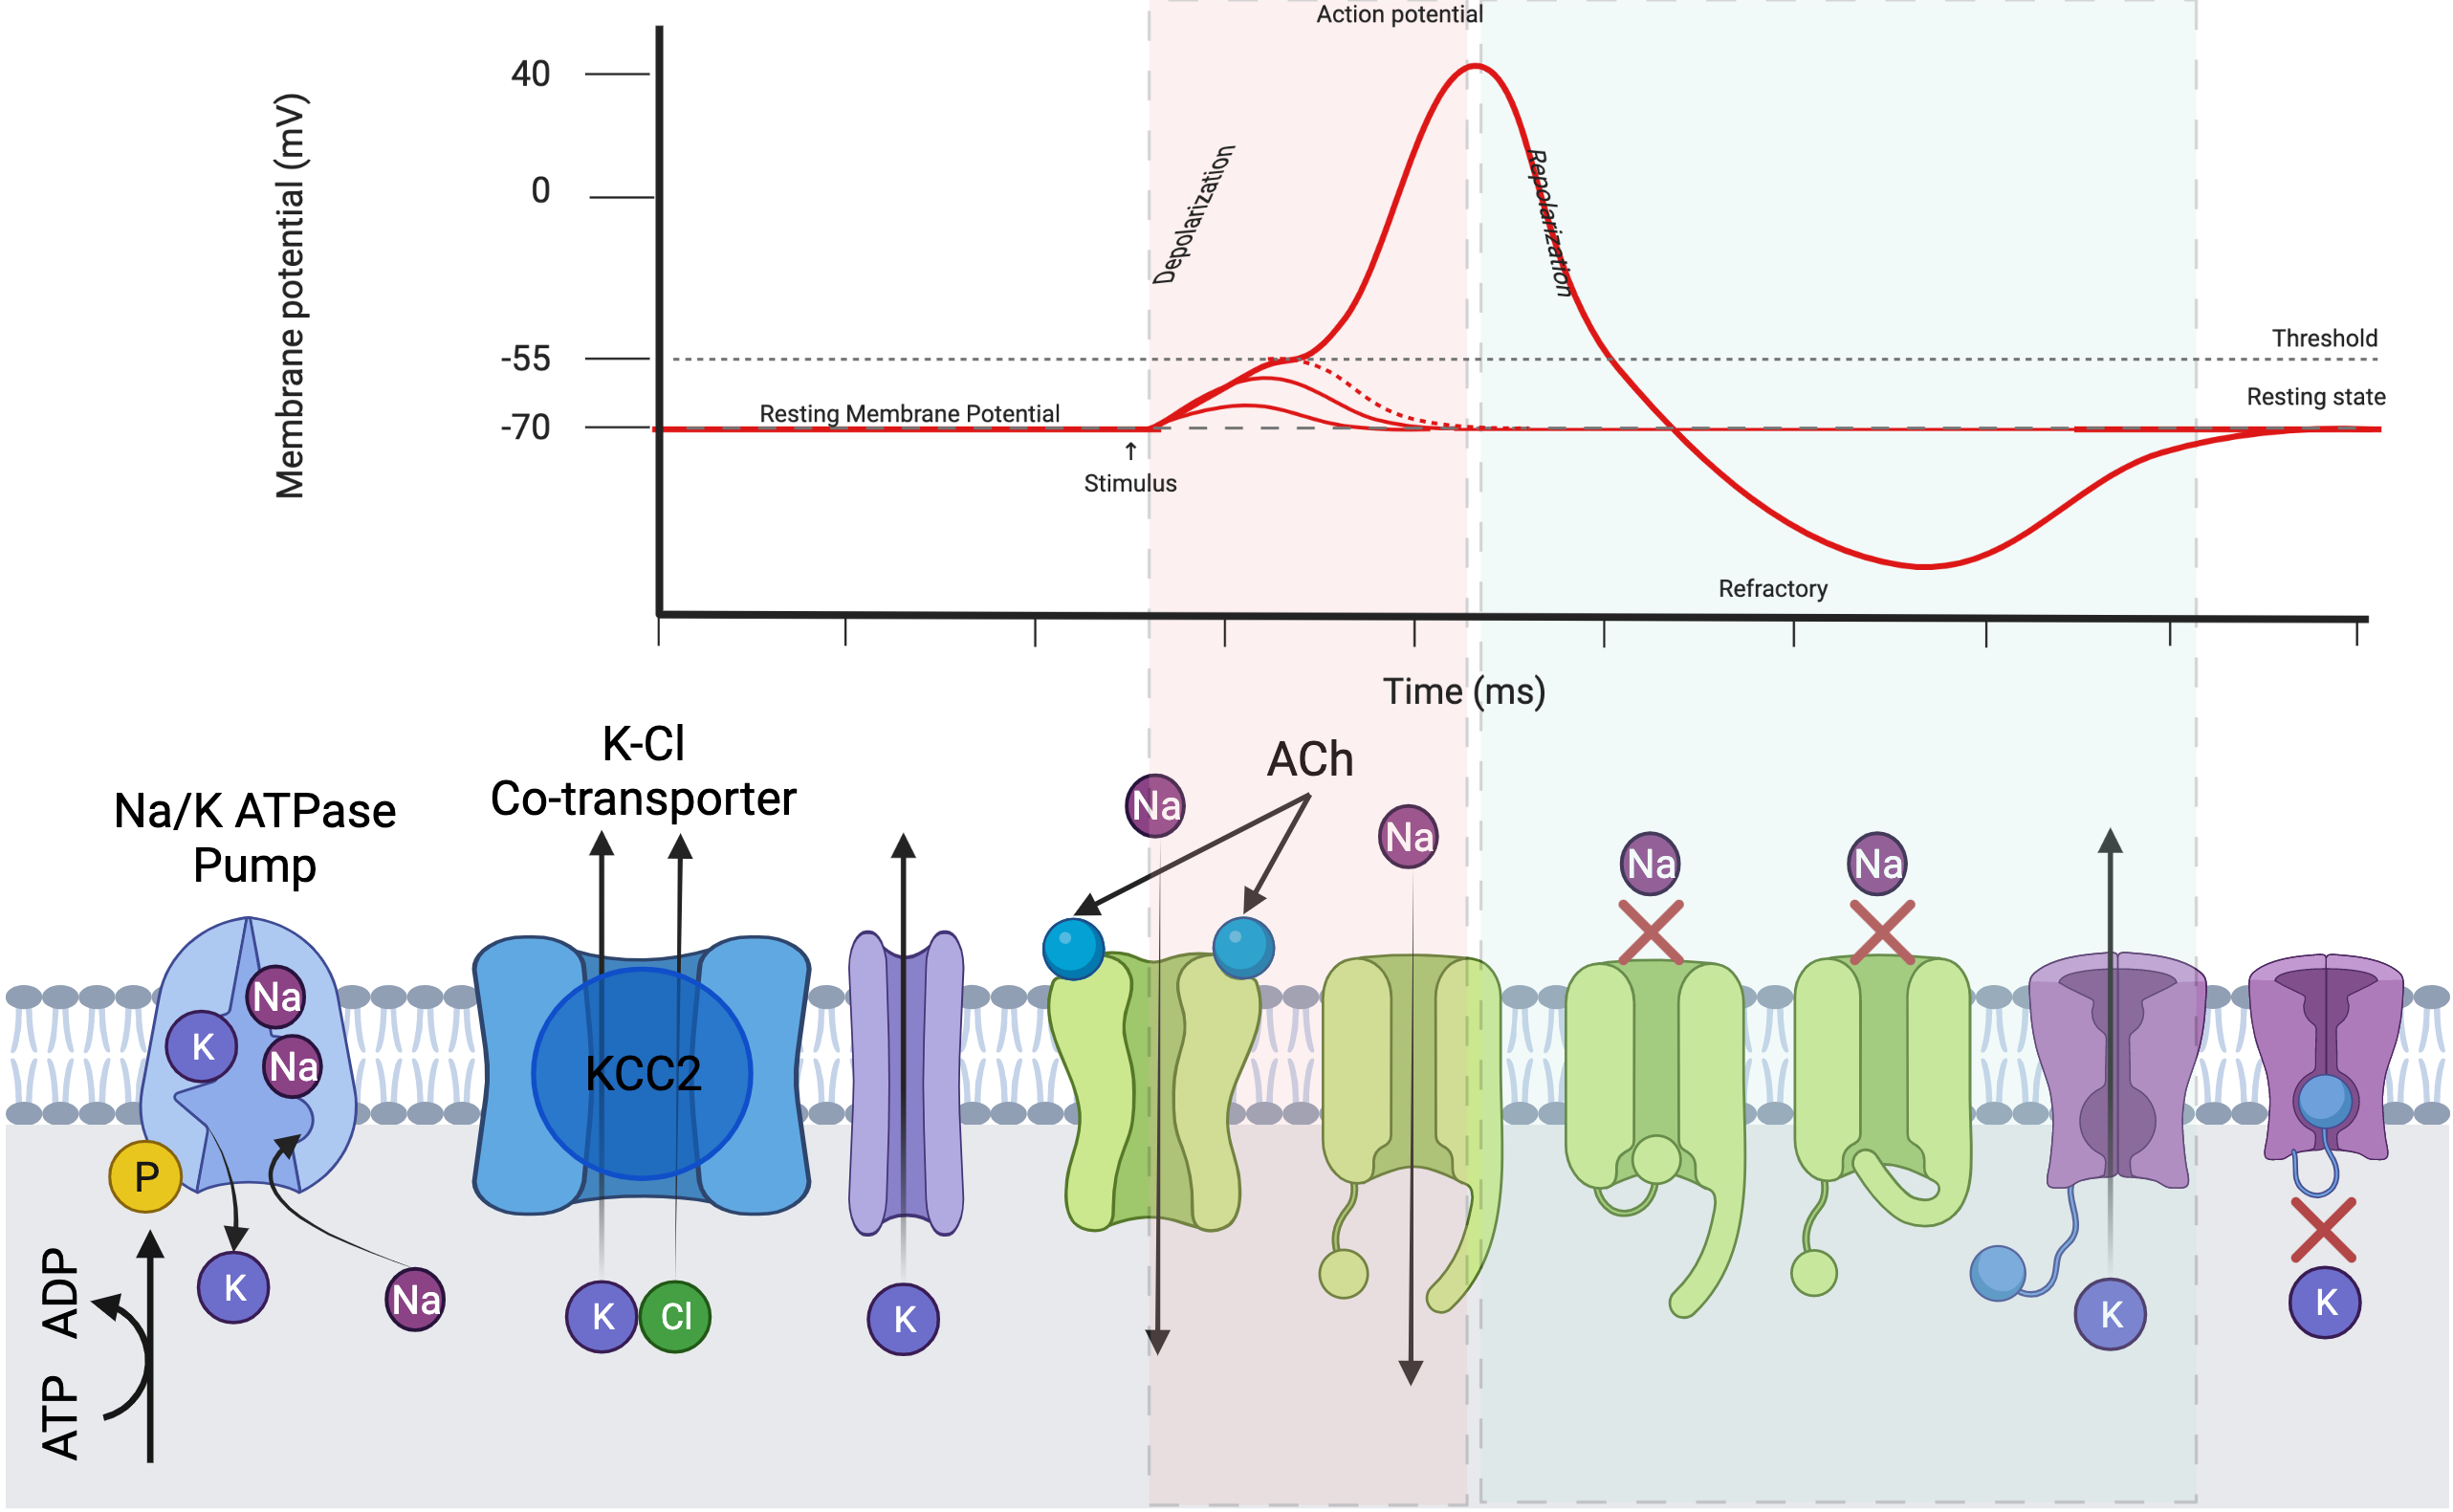
\includegraphics[width=1\linewidth]{./figure/cell_membrane.png}
    \caption{Cell Membrane Components and their general contribution to RMP and an AP \footnotesize{Created with BioRender.com}}
    \label{fig:cell_membrane}
\end{figure}


\paragraph{Pumps \& Transporters}
$Na^+/K^+$ ATPase pumps are embedded throughout excitable membranes. These protein based molecular machines convert the energy of ATP to the movement of three $Na^+$ outside the cell and two $K^+$ inside the cell with each cycle of the pump (each use of ATP). Given the natural tendency of molecules to move based on a concentration gradient (high concentration to low concentration) the resultant higher concentration of  $Na^+$ outside and higher concentration of $K^+$ inside the cell requires the work of these active transport pumps against the concentration gradient.
The $K^+$ - $Cl^-$ co-transporter (KCC2) utilizes the $K^+$ concentration gradient created by the $Na^+$/$K^+$ ATPase pumps to move $Cl^-$ out of the cell as an exchange with $K^+$.


%\begin{figure}
%    \centering
%   \includegraphics{.\figure/pumps.png}
%    \caption{$Na^+/K^+$ ATPase Pumps \footnotesize{Created with BioRender.com}}
%    \label{fig:pumps}
%\end{figure}


\paragraph{Channels \& Receptors}
Channels are proteins embedded in the cell membrane that allow passage of molecules between the intracellular and extra cellular space. Channels can be gated and therefore only allow passage under certain circumstances. 

Voltage gated channels only allow passage when the membrane potential is at certain values. They may open at a certain value and close a certain period of time later; or they may close at a certain value and open a period of time later. 
Ligand gated channels only allow passage when the channel is activated due to the binding of a ligand (a molecule that can bind). A ligand gated channel is also a receptor, or closely associated with a receptor. 

$Na^+$ channels allow the passage of $Na^+$ with its concentration gradient and can be either ligand gated or voltage gated. $K^+$ channels allow the passage of $K^+$ with its concentration gradient and in nerve and muscle excitable membranes are both non gated and voltage gated. Cl channels allow the passage of $Cl^-$ along its concentration gradient and in the sarcolemma are not gated ($Cl^-$ channels are not depicted in \ref{fig:cell_membrane}, but would resemble the $K^+$ channel to the far right of the figure.).

Receptors are proteins that allow ligand binding. Some receptors are ligand gated channels (a receptor where the activity that binding produces is opening a channel gate). Other receptors perform different activities within the cell. 

%\begin{figure}
%    \centering
%    \in$Cl^-$udegraphics{.\figure/receptors.png}
%    \caption{Receptors \footnotesize{Created with BioRender.com}}
%    \label{fig:receptors}
%\end{figure}

\subsection{Establishing the Resting Membrane Potential}

For our purposes the process of establishing the RMP in the sarcolemma focuses on roles played by the concentration gradients and electrical potential created by $Na^+$, $K^+$ and $Cl^-$. Each of these elemental molecules exist in the body as ions (they carry a charge based on whether the have too many electrons ($Cl^-$) or two few electrons ($Na^+$, $K^+$).\footnotemark\footnotetext{Ca is an ion that has 2 more protons than electrons (hence the 2+ superscript in its abbreviation).} 

\subsubsection{Electrical Potentials \& Equilibrium Potential}

% Consider adding Nernst, and Goldman's equations

Movement of molecules across the cell membrane is influenced by the concentration gradient of the ion across the membrane, the permeability of the membrane for that ion and the and the electrical equilibrium potential across the membrane. When we describe electrical potentials the convention is to speak from inside the cell (intra cellular). A negative potential means at the membrane inside the cell there is a negative charge. A positive potential means that at the membrane inside the cell there is a positive charge. We can, for the sake of understanding, simply invert this and say a negative potential means that at the membrane OUTSIDE the cell has a positive charge; and that a positive potential means that at the membrane OUTSIDE the cell has a negative charge.

When an ion moves across a membrane it carries a charge and creates an electrical potential. An important point is that the electrical potential created at the membrane is not created by the concentration gradient, but from the movement of ions which is based on the concentration gradients.  The $Na^+$/$K^+$ ATPase pumps work at a rate in response to the concentration gradients (speed up if there is a need to, slow down to resting levels when able). But even for long periods of high frequency excitations there is no risk of significant change to the ionic concentrations outside or inside the cell. Thinking that there an absolute change in ionic concentration is required for an action potential is a common misconception about action potentials\cite{silverthorn_uncovering_2002}. When $K^+$ moves across the membrane (out of the cell) it creates a negative potential. When $Na^+$ moves across the membrane (into the cell) it creates a positive potential. When $Cl^-$ moves across the membrane (into the cell) it creates a negative potential. 

To generalize these facts. When a positive ion moves into the cell it creates a positive potential; when it moves out of the cell it creates a negative potential. When a negative ion moves into a cell it creates a negative potential; when it moves out of a cell it creates a positive potential. These potentials are based on the movement of the ions, not on their concentration. 

The electrical potential created at the membrane by the movement of an ion then has an influence on the movement of ions. The negative electrical potential created at the membrane by the movement of $K^+$ out of the cell will eventually resist the continued movement of $K^+$ out of the cell. How negative that negative potential needs to be to stop the movement of $K^+$ out of the cell is dependent on the concentration gradient.\footnotemark\footnotetext{It is also dependent on the temperature (which is kept within tight boundaries in the body), Faraday's constant, and the universal gas constant. From these variables the potential generated by any ion can be determined with the Nernst Equation, which is not be covered here at this time.} The electrical potential that stops the movement of an ion is called the \textbf{equilibrium potential}. Figure \ref{fig:equilibrium_potential} shows the concentration gradient and resultant equilibrium potential for our primary ions of interest ($Na^+$, $K^+$, $Cl^-$). Each equilibrium potential in \ref{fig:equilibrium_potential} is based on the assumption that it is the only ion moving across the membrane. In reality they are all moving across the membrane with varying rates which are based on the permeability of the membrane to each ion at any moment in time.\footnotemark\footnotetext{The Goldman-Hodgkin-Katz (GHK) Equation (model) allows the estimation of the membrane potential based on $Na^+$, $K^+$, $Cl^-$ concentration gradients and membrane permeability (along with several other relevant variables. A calculator for the GHK Equation can be found at \url{https://www.physiologyweb.com/calculators/ghk_equation_calculator.html}.}

\begin{figure}[!ht]
    \centering
    %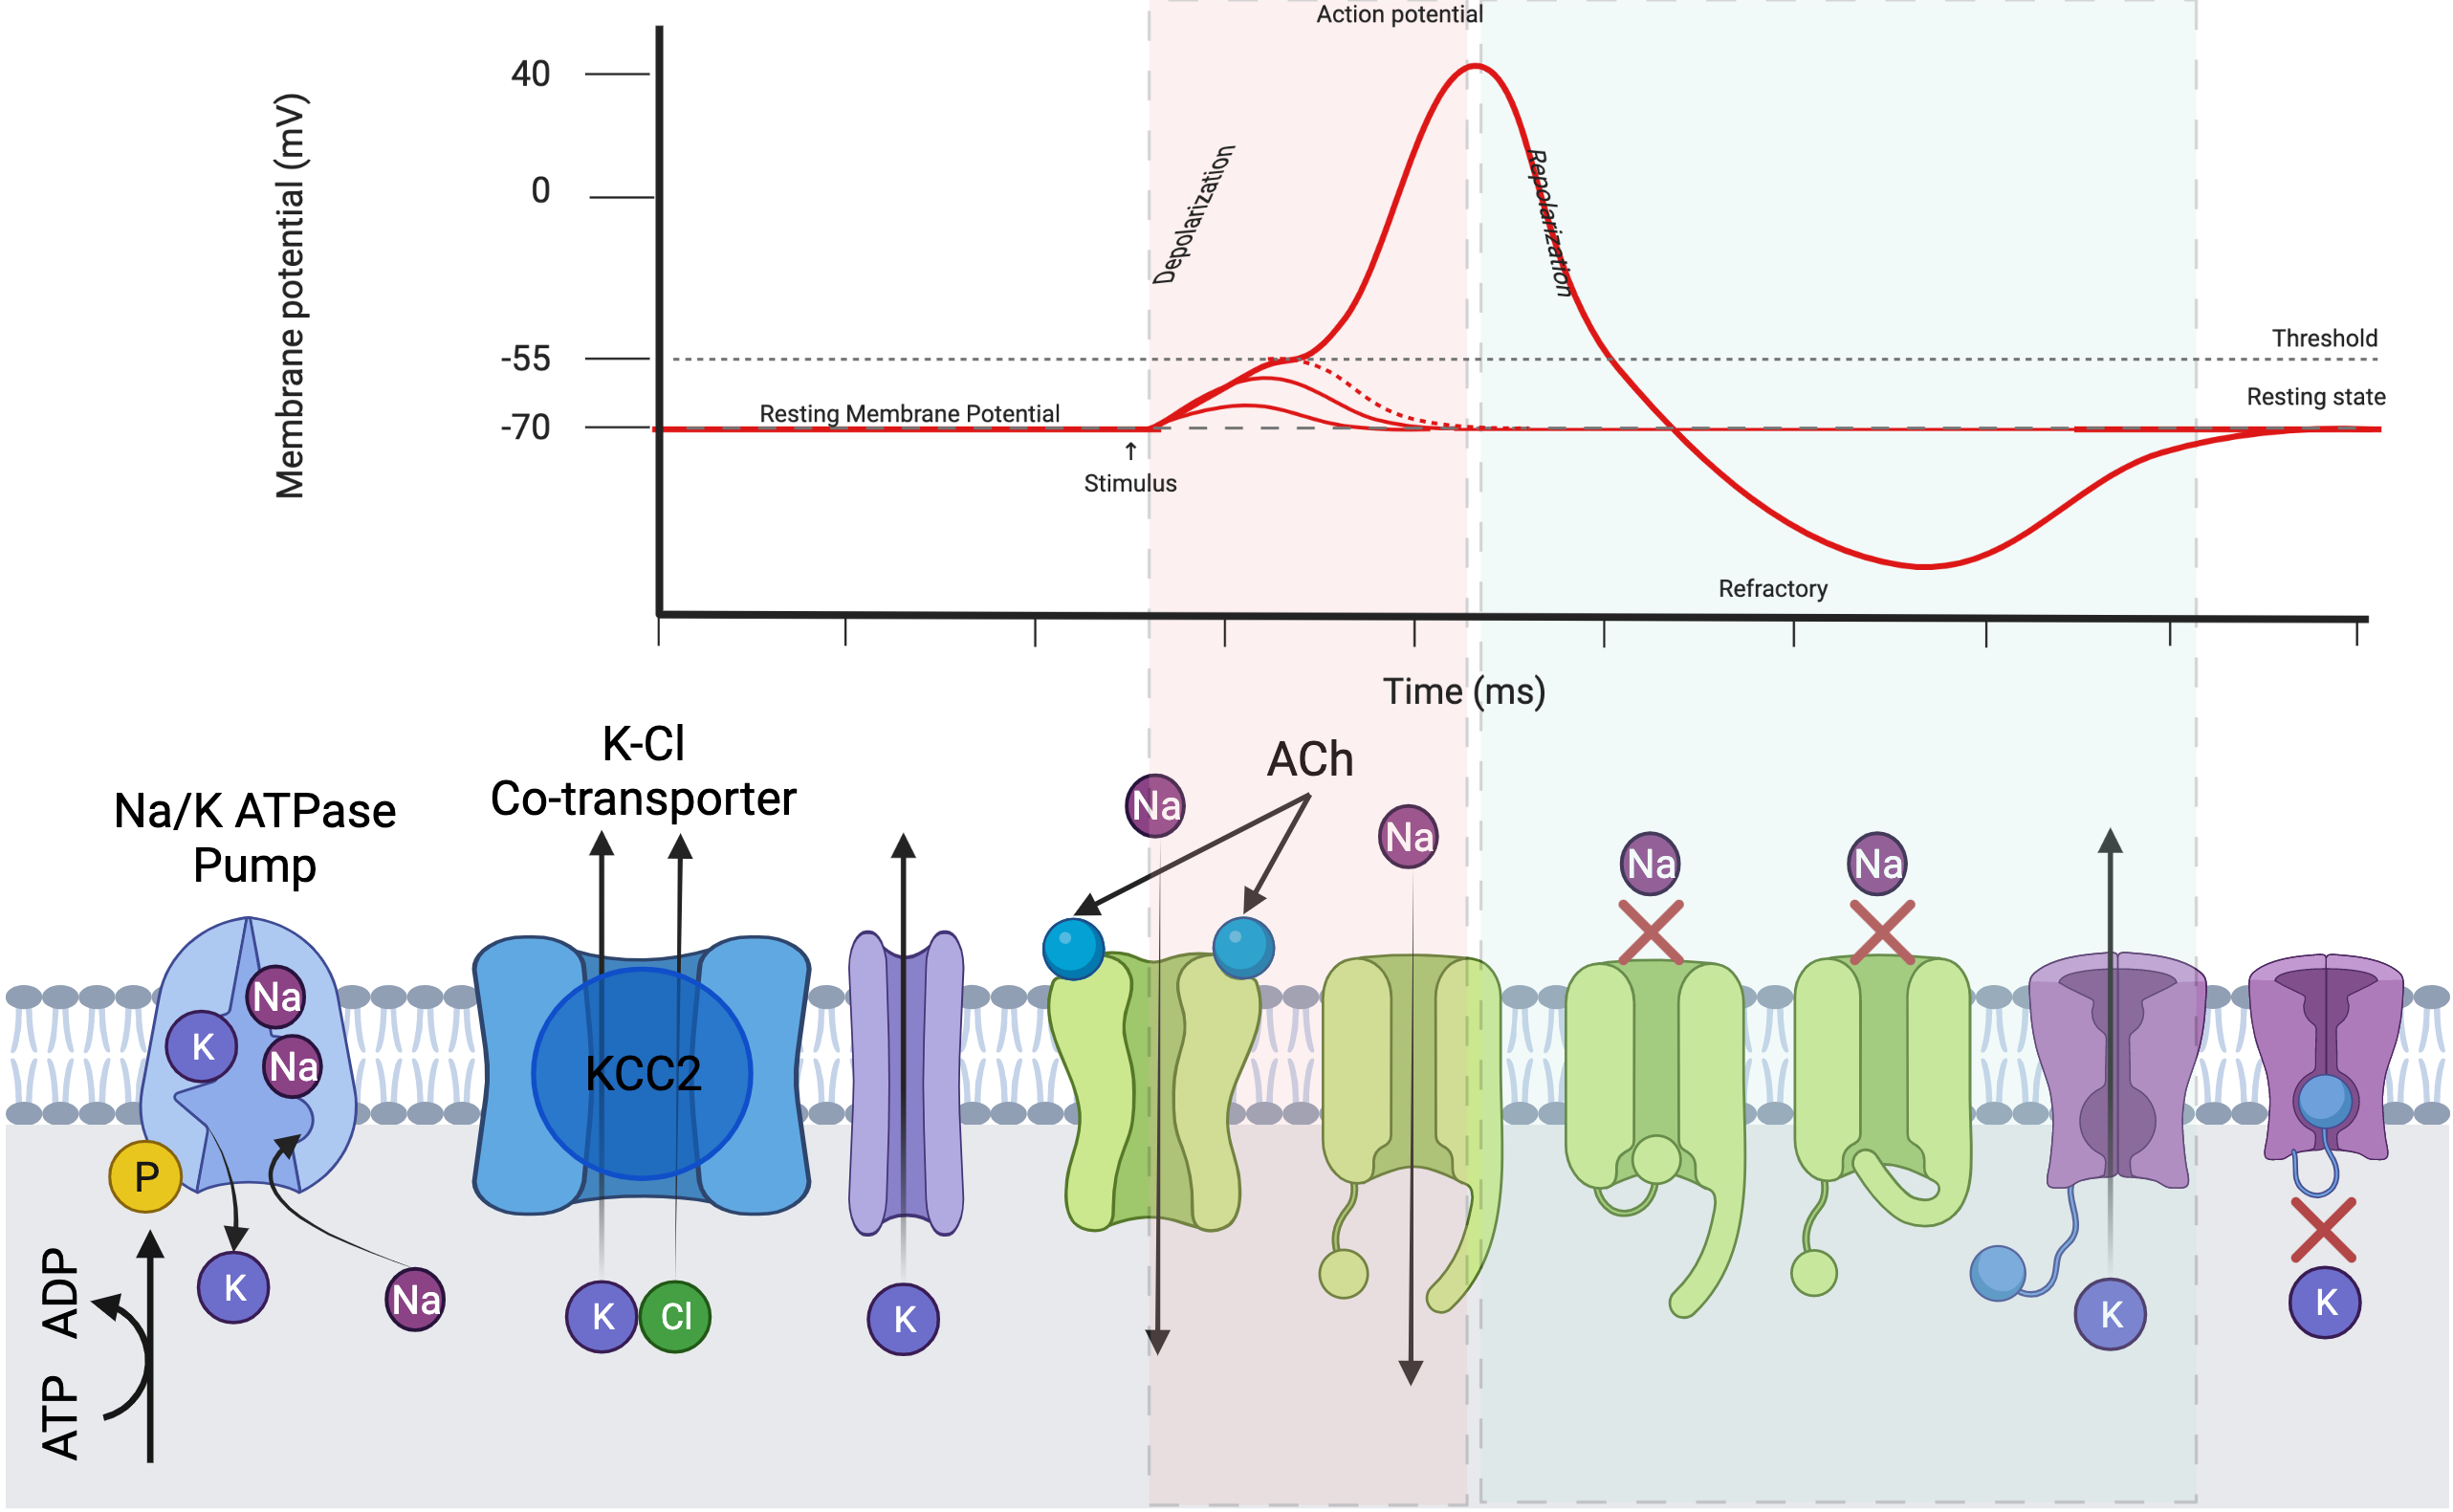
\includegraphics[width=1\linewidth]{./figure/cell_membrane.png}
    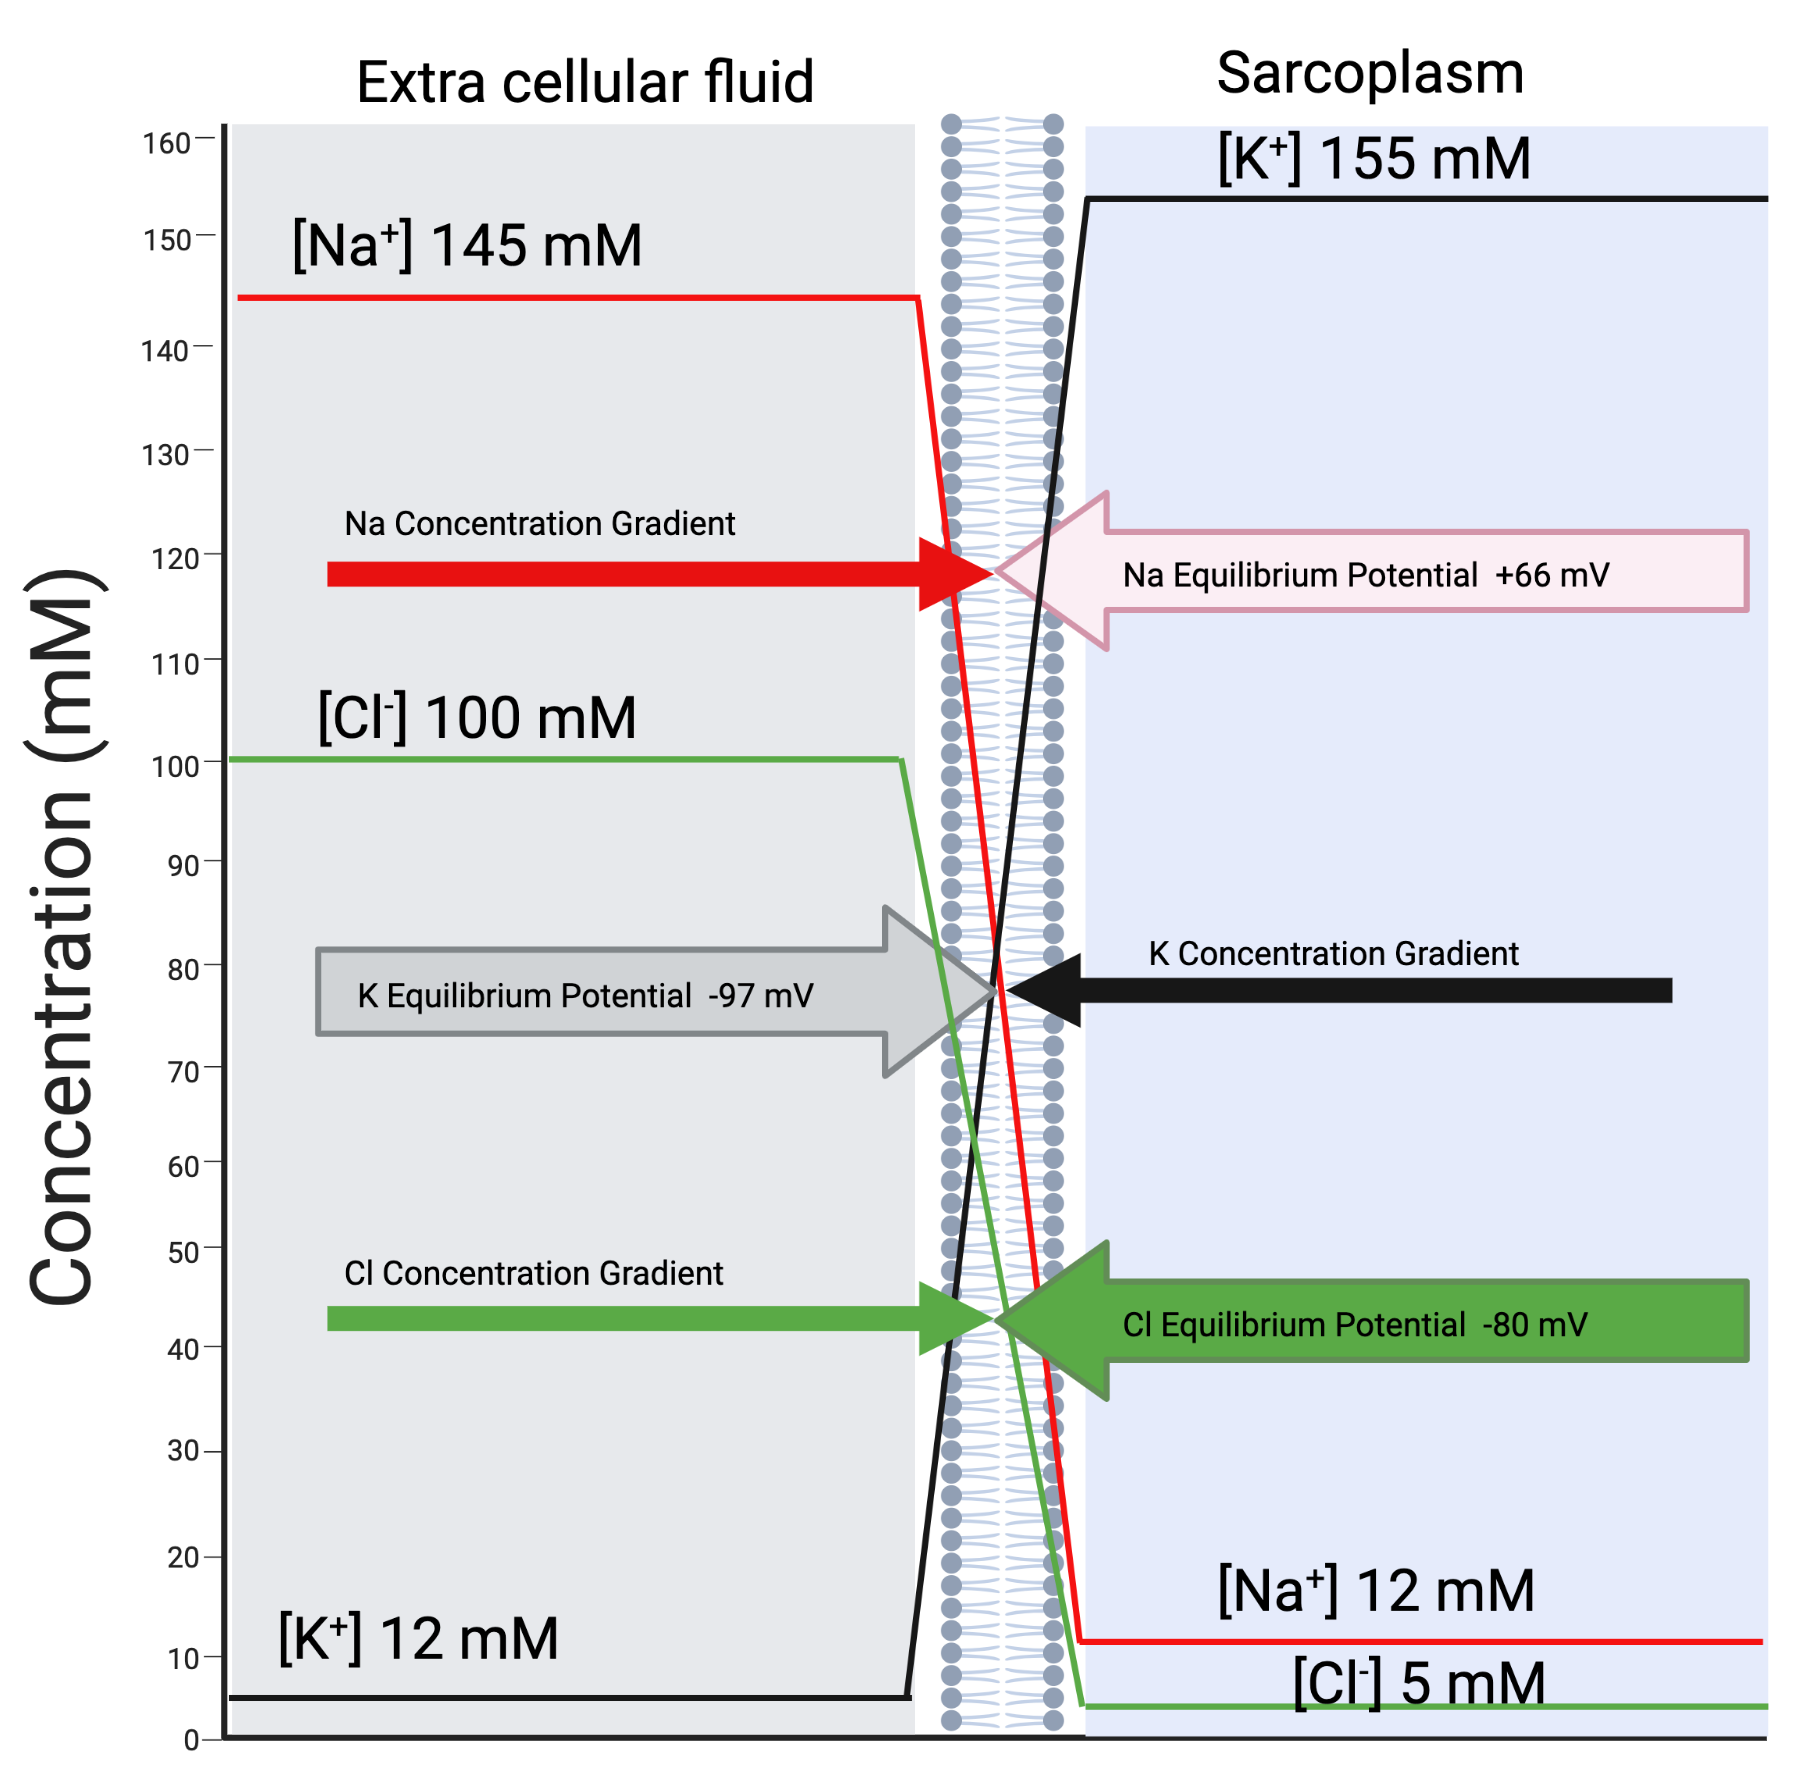
\includegraphics{./figure/equilibrium_potential.png}
    \caption{Generation of Equilibrium Potentials \footnotesize{Created with BioRender.com}}
    \label{fig:equilibrium_potential}
\end{figure}

\paragraph{}
The resting membrane potential is an equilibrium potential. It is the consequence of two physiological situations. First, the presence of large concentration gradients for $K^+$, $Na^+$  and $Cl^-$ across the membrane. Second, the relative permeability of the membrane to these ions. For example, based on Figure \ref{fig:equilibrium_potential}, if $K^+$ was the only ion that the membrane was permeable to at rest the RMP would be equal to the $K^+$ equilibrium potential (about -97 mV).

The concentration gradients for $K^+$ and $Na^+$ are established primarily by the $Na^+$-$K^+$-ATPase pumps. The concentration gradient maintains a large outwardly directed $K^+$ gradient, and a large inwardly directed $Na^+$ gradient. The concentration gradient for $Cl^-$ is maintained primarily through the actions of a $K^+$ - $Cl^-$ co-transporter known as KCC2. Relative to the other ions, there is a moderate inwardly directed $Cl^-$ gradient.

%Change the figure to reduce the size of the gradient vector for Cl-

Since these ions do not pass through the lipid bi-layer of the cell membrane the permeability of the membrane to each ion is tuned by the presence of ion specific channels. Therefore, the relative permeability of the plasma membrane to $Na^+$, $K^+$ and $Cl^-$ is dependent on the number and state (open or closed) of ion-selective membrane channels. Different membranes display different degrees of permeability to different ions, and due to gating mechanisms on many of the ion-selective channels the permeability can be changed (this is a hugely important point considering the entire purpose of an RMP (polarization) is to have the opportunity to generate an AP (depolarization)).

In resting conditions the membrane of nerve and muscle cells are most permeable to $K^+$. In addition to KCC2 allowing movement of $K^+$ out of the cell, there are also non-gated $K^+$ specific ion channels. When combined with the relatively high permeability of $K^+$, the concentration gradient results in a $K^+$ flow out of the cell. As $K^+$ flows out it creates a negative electrical potential. However, the negative electrical potential resists further flow of $K^+$ outside of the cell (and eventually reaches an equilibrium potential). Since $K^+$ has the highest permeability at rest, the resting membrane potential is primarily influenced by the equilibrium potential of $K^+$. It is important to note that while there is no net flow of $K^+$ at the $K^+$ equilibrium potential, $K^+$ is still flowing out of the cell and continues to generate the negative membrane (equilibrium) potential, and $K^+$ continues to be pumped into the cell by the $Na^+$/$K^+$ ATPase pumps. The term "equilibrium" for equilibrium potential means equilibrium in flows (no net flow, no net gain in or outside the cell).

Note from Figure \ref{fig:equilibrium_potential} that the equilibrium potential of $Cl^-$ is close to $K^+$. The implication is that $Cl^-$, despite its concentration gradient encouraging inward flow, does not at RMP, have net inward flow. $Cl^-$ has a higher permeability than $Na^+$ at rest, but a much lower permeability than $K^+$. An important attribute about $Cl^-$ for the sarcolemma and axon membranes is that the permeability of the membrane does not change much, even during an AP. This contributes to the stability of the RMP and helps prevent recurrent self excitation in these membranes.

The equilibrium potential of $Na^+$ is positive (opposite of $K^+$ and $Cl^-$). At RMP the permeability for $Na^+$ is very low, and therefore $Na^+$ has very little impact on the RMP. The importance of $Na^+$ starts when gated $Na^+$ channels start to open - that's when the action begins.

% Old text - don't delete yet
% Under normal, healthy, conditions different cell membranes have slightly different resting membrane (equilibrium) potentials. These differences are due to differences in the permeability of the membranes to $K^+$ (or to other ions, such as $Na^+$, $Cl^-$, $Ca^{2+}$). The extra cellular concentration of these ions is held constant throughout the body and therefore under normal circumstances differences in the concentration gradients are not a major source of differences in resting membrane potentials. 

\subsection{Trigger \& Spread of Sarcolemma Excitation (AP)}

As can be noted in Figure \ref{fig:equilibrium_potential} the equilibrium potential for $Na^+$ is positive. When the membrane relative permeability for $Na^+$ increases (becomes greater than $K^+$ and $Cl^-$) the membrane potential starts to depolarize and even to switch to a positive polarity. This is an action potential. At the molecular level, an action potential is the sudden increase in relatively permeability of the membrane to $Na^+$.  

\paragraph{Triggering the Action Potential (Initial Excitation)}
The events leading to an action potential on the sarcolemma are initiated by the opening of ligand gated $Na^+$ channels by the binding of ACh to these receptors at the motor end plate. The micro potentials created by the opening of the ligand gated $Na^+$ channels by the binding of ACh then open voltage gated $Na^+$ channels due to a change in voltage in the membrane potential (becoming less negative). The number of voltage gated $Na^+$ channels that open is proportional to the change in the membrane potential. This cycle of opening in response to a voltage change is self perpetuating since once a $Na^+$ channel opens $Na^+$ flows into the cell due to the $Na^+$ concentration gradient. Due to the movement (not a change in the actual gradient) the membrane potential voltage changes (becomes less negative) as the potential moves toward the $Na^+$ equilibrium potential. The point that approximately half of the voltage gated $Na^+$ channels open is considered a threshold potential. At the threshold potential the voltage gated $Na^+$ channels continue to rapidly open until the equilibrium potential approaches that of $Na^+$ (as opposed to $K^+$) since at this point the membrane is more permeable to $Na^+$. The equilibrium potential for $Na^+$ is approximately 66 mV.  Once a membrane reaches the threshold potential an action potential is inevitable. It is at this point that the action potential is said to be “all or none.” Prior to the threshold potential membranes can undergo micro potential changes. These micro potentials can be depolarizing (excitatory potentials that move the membrane potential toward the threshold), or hyperpolarizing (inhibitory potentials that move the membrane potential further away from the threshold potential). The use of micro potentials to regulate muscle tension is an important part of Chapter \ref{chp:regulation} since it is a process that occurs at the $\alpha$-motor neuron dendrites in the spinal cord, not at the NMJ.\footnotemark\footnotetext{An $\alpha$-motor neuron, once excited, will release only one neurotransmitter, ACh at its axon terminal. ACh will only have one effect at the NMJ, creating excitatory micro-potentials on the motor end plate. However, in the Central Nervous System (such as the Spinal Cord) competing neurotransmitters can be released at synapses of the $\alpha$-motor neuron dendrites. The impact of these neurotransmitters can be excitatory or inhibitory. Since they occur after the synaspse they are called excitatory post synaptic potentiations (EPSPs) or inhibitory post synaptic potentiations (IPSPs). Whether, and how frequently, an $\alpha$-motor neuron sends an excitation to the muscle fibers it innervates is balanced by competition between the EPSPs and the IPSPs.}

\paragraph{Spread of the Action Potential (Wave of Excitation)}

The wave of excitation of the AP across the sarcolemma and T-tubules occurs due to the self-perpetuating opening of voltage gated $Na^+$ channels. When a region of the membrane depolarizes it opens the nearby voltage gated $Na^+$ channels which depolarize that region, which then opens the nearby voltage gated $Na^+$ channels which depolarize that region, "And so it goes."\footnotemark\footnotetext{A quote for other Kurt Vonnegut fans.)}

Of course, there cannot be an AP if there is no RMP. Therefore, the AP must end. The membrane must repolarize to be ready for another depolarization. Considering muscle tension is, partly, regulated by how frequently it experiences excitation (which can reach upwards of 180 Hz, that is 180 excitations per second, for those excitations to occur there need to be an equal number of repolarizations).

The process of repolarization occurs in two steps. Voltage gated $Na^+$ channels have two gates. One is an activation gate and it is closed under resting conditions and opens during excitation. The second is an inactivation gate and it is open under resting conditions but closes soon after the activation opens. The inactivation gate closure is timed, it is not triggered by events outside of the molecule itself. Closing the inactivation gate is the first step to stopping an action potential. The closure of the inactivation gates reduces the relative permeability of $Na^+$. While the activation gate is open and the inactivation gate is closed the membrane is in the absolute refractory period (cannot undergo depolarization regardless of how great an excitation stimulus may be). To be reset and completely ready for another action potential the activation gate must close and the inactivation gate must open (these are timed events).

The second step (really second part, do not think of these in an overly temporal manner since events overlap in time) to repolarization is opening of voltage gated $K^+$ channels. These are delayed (take longer to open than the voltage gated $Na^+$ channels). Once the voltage gated $K^+$ channels open the membrane permeability to $K^+$ increases higher than under resting conditions which further expedites the repolarization process and can also result in a hyper polarized state (slightly more negative membrane potential than the normal resting membrane potential). Closing the voltage gated $K^+$ channels is also a timed event. While they are open the membrane is in a relative refractory period. It is resistant to excitation, however, with an increased stimulus it can be excited.

The overall process of repolarization and return to the resting membrane potential takes approximately 3-4 milliseconds (ms). Assuming 3 ms is the fastest interval for another AP, the upper limit on excitations would be approximately 333 Hz (which exceeds the maximum capacity for muscle fiber twitches per second).

Spread of excitation occurs in one direction (meaning it does not result in cyclic repeating action potentials of the entire membrane) because of the refractory periods. If a membrane is visualized as a set of dominoes and the resting potential is when the dominoes are upright, and an action potential is when a domino falls, then the refractory period is the period when the domino is still fallen. Because of the fallen domino on one side of the next falling domino, the dominoes fall in one direction away from the starting stimulus. A further safeguard against cyclic repeating actions potentials in the sarcolemma is the constant permeability for $Cl^-$ in the sarcolemma. Recall that at RMP $Cl^-$ has no net flow because its equilibrium potential is near the $K^+$ potential. When the membrane potential fluctuates away from the the $K^+$ (and $Cl^-$) equilibrium potential there is net movement of $Cl^-$. This $Cl^-$ net movement (into the cell) contributes to repolarization but also to stability of the RMP in the moments following an AP. In situations such as myotonia congenita altered membrane $Cl^-$ permeability leads to a higher occurrence of myotonia (sustained muscle tetany) due to recurrent muscle excitation from cyclic repeating action potentials \cite{adrian_action_1976}.

\subsection{Excitation to Regulation}

This section has taken a deeper dive into the molecular events of excitation than the previous section. It should be clear that many events must occur for one excitation, particularly since one excitation creates a twitch, and a twitch is not enough to produce meaningful movement. A more efficient system of excitation-activation coupling exists in the cardiac muscle. However, in the skeletal muscle the efficiency of creating tetany from one excitation is sacrificed for the sake of regulation of muscle tension. Since creating tetany requires many action potentials, then the amount of tetany, and therefore the amount of tension, can be regulated by the number of action potentials. The regulation of muscle fibers is the topic for Chapter \ref{chp:regulation}.


\section{\textit{Clinical Physiology Connections}}

The concepts of excitable membranes, receptors, ligand channels and signal transduction are pervasive throughout clinical physiology. This final section of the chapter introduces some clinical physiology connections that are now possible given your understanding of excitable membranes, including the neuroendocrine system, sensory receptors and pharmacodynamics. These topics return throughout the book in particular contexts.

\subsection{Neuroendocrine}

The neuroendocrine system regulates several critical physiological systems and coordinates cellular functions throughout the body. Examples include mobilizing the body for fight or flight reactions by getting all cells in the body ready to meet demands that require energy mobilization at the expense of other maintenance activities. For example, release of hormones for fight or flight signals liver cells to hold off on using energy to maintain the cell membrane and instead use energy to convert glycogen (a stored fuel) into glucose (a usable fuel). The neuroendocrine system can alert cells all over the body to do activities that each of those cells can do for the fight or flight situation, even though those activities are varied between the cells. While the liver cells are releasing glucose, the heart cells are prepared to use more glucose and are working more frequently (higher rate) and harder (more pressure). The differentiation and variety of tasks completed by these cells is due to the specialization of the cells, and due to the receptors around the body that are responding to the same ligand. Most cells in the body have a ligand receptor for epinephrine (a major catecholamine of the fight or flight response). Epinephrine is also called adrenaline. Receptors for epinephrine are therefore called adrenergic receptors. The adrenergic receptors on all cells have a similar binding location for epinephrine, but the receptor itself transducts different signals into the cell depending on the receptor and depending on the cell. For example, the adrenergic receptors on smooth muscle in arterioles in the systemic circulation signal contraction which results in vaso-constriction. However, the adrenergic receptors on smooth muscle in bronchioles in the lung signal relaxation, which results in broncho-constriction.

The fight or flight (alert) response from the neuroendocrine is a coordinated response of the component of the central nervous system called the autonomic nervous system, and in particular the sympathetic nervous system (SNS). The SNS is a truly neuroendocrine system because it has both nervous system and endocrine components. Ligands for the SNS, epinephrine and norepinephrine, are also both neurotransmitters and hormones.

For homeostasis (balance), if there is a fight or flight (alert) system then there should also be a rest, digest and reproduce (chill) system. The chill system is the parasympathetic system (PNS). The PNS is a nervous (but not neuroendocrine) system. The connections through the body of the PNS are all mediated with nerve function and neurotransmitters (not endocrine, or hormone signals). This is not to say that the during a chill situation hormones are not involved. Just that if there are pathways through which the PNS mediates those chill (rest, digest, reproduction) hormones they have not been discovered yet (at least as far as the author knows as of \today). The primary neurotransmitter for the PSN is acetylcholine (ACh). The PNS receptors that bind ACh are called cholinergic receptors. 

\subsection{Sensory Receptors}

Sensory receptors are specialized receptors at the terminal end of the axon of a sensory neuron. They differ from ligand and voltage gated receptors in the signals that provokes their excitation. When a sensory receptor is excited it sends an afferent signal (to the central nervous system, as opposed to efferent signal, away from (or exiting) the central nervous system). In general, the signal the provokes excitation in a sensory neuron is whatever phenomenon or sensation that sensory neuron is associated. If the sensory neuron is excited by changes in temperature then it is a temperature sensory neuron; if by changes in tension, it is a tension sensory receptor; if by vibrations, it is a vibration (as in the ear) sensory receptor; if by photons, it is a light sensory receptor (as in the retina); if by certain chemicals or ions (such as $H^+$ for pH, or carbon dioxide, or oxygen) they are chemoreceptors; if by changes in pressure they are baroreceptors. Some sensory receptors terminate in areas of the brain that allow perceptions of the signal in a way that gives them additional meaning. For example, some chemoreceptors proceed to the brain and produce pain signals, once in the brain a complicated cascade of connections are made that can, over time, change from being protective to themselves harmful to movement. Other chemoreceptors that detect an increase in carbon dioxide proceed to areas in the nervous system to produce unconscious reflex responses (changing respiratory rate) and also to the brain (a general state of anxiety and air hunger). Some receptors don’t go to the brain at all, but interact at areas in the nervous system where responses are automatic (baroreceptors as part of the autonomic nervous system to regulate blood pressure). Since baroreceptors don’t go beyond the brain stem we do not perceive what our blood pressure is directly - making elevated blood pressure a “silent killer.” To be a homeostatic regulatory system there needs to be a sensory receptor of some type that contributes to the monitoring of the homeostatic variable. So a homeostatic regulatory system includes a homeostatic variable that is sensed by a sensory receptor that sends an afferent signal to be processed (often not perceived), which then sends an efferent signal to exert an action which aims to adjust the homeostatic variable. The neuroendocrine system is commonly involved in such systems, receiving afferent signals, and sending efferent signals. Most physiological homeostatic systems are negative feedback systems, which means sensation of an increase in a variable triggers response to decreases that same variable (and vice versa).

\subsubsection{Sensory Receptor Dynamics}
Sensory receptors are proteins embedded in cell membranes. Therefore, the cell has control over some dynamic and important behavior of these receptors (indeed, all receptors).  Up-regulation is a term for sensory receptor dynamics that includes an increase in the number of receptors. Down-regulation is a term for sensory receptor dynamics that includes a decrease in the number of receptors. With up-regulation or down regulation there are changes to the strength of a excitation and therefore signal sent to the respective neurons. For example, with up-regulation of chemoreceptors for carbon dioxide an individual will have a higher respiratory rate and maintain a lower carbon dioxide level since their response to carbon dioxide is increased. The up-regulation then continues to propagate itself. Since it results in lower carbon dioxide levels, the receptors remain up-regulated in an attempt to be able to respond to the lower carbon dioxide levels. A balance point is eventually achieved. But this new balance point may be enough to result in what is converted altered homeostasis. In individuals taking a beta-blocker (beta-adrenergic blocker medication) the lack of cardiac response to neuroendocrine stimulus results in higher adrenaline levels. The adrenergic receptors of the heart down-regulate in response to higher circulating adrenaline which further blunts cardiac responsiveness to adrenergic stimulation. A balance point is eventually achieved as with the previous example, however, the individual has an alteration to homeostasis. 

\subsubsection{Neuromuscular Sensory Receptors} 
There are several important neuromuscular sensory receptors that sense signals from the muscle, musculotendonous junction and/or the tendon. Signals for tension (such as golgi tendon organs), signals for changes in length (such as the muscle spindle), and signals for the chemical constituents of the extra cellular fluid surrounding muscle fibers (chemoreceptors). These receptors and their role in muscle function is covered in upcoming chapters on regulation, energetics and micro-circulation.

\subsection{Pharmacodynamics}

Pharmacology is divided into pharmacotherapeutics and toxicology. Toxicology focuses on the harmful effects that chemicals, such as medications, may have on the body. Pharmacotherapeutics is the development and study of medications. Pharmacotherapeutics is divided into pharmacokinetics and pharmacodynamics. Pharmacokinetics focuses on the absorption, distribution and metabolism of medications. Pharmacodynamics focuses on the intended systemic and cellular effects of medications. Pharmacodynamics is therefore a study of the actions of medications in the body. The cellular and systematic effects of a medication is often related to what receptors it binds, what neurotransmitter or hormone it effects of mimics, or what signal transduction mechanism it influences. Pharmacodynamics often includes changes to the process of excitation discussed in this chapter.

\subsubsection{Curare}
Curare is paralyzing agent. It stops the excitation of the motor end plate. It does so by competitively and reversibly binding to ACh receptors on the motor end plate which blocks those receptors from binding with ACh. When curare binds to an ACh receptor it does not open the ligand gated $Na^+$ channel and therefore prevents the initiation of depolarization. As a competitive binding, curare blocks the ACh receptor and thus inhibits the ACh binding and response. Another term for competitive binding is that curare is an antagonist (blocks without producing an effect). Some medications are agonists, they bind and create an effect and are thus utilized to facilitate additional cellular activity beyond that of the normal ligand. As a reversible binding medication, curare can be removed from the ACh receptor. Medications can also create irreversible binding. Curare is also selective, it only binds to skeletal muscle motor end plate ACh receptors. Which means it selectively inhibits these receptors and not other ACh receptors throughout the body. This means the systemic response is limited to skeletal muscle paralysis. If used during surgery without other anaesthetics it would produce paralysis but no change in pain sensation, a very unpleasant surgery that would be stopped when the pain and anxiety of the procedure produced a rapid heart rate and rising blood pressure due to the fight or flight response of the neuroendocrine system (which would not be stopped by curare). In addition to surgical or intensive care situations, curare can be used as a poison, causing death by asphyxiation since the muscles of ventilation (breathing) are skeletal muscles. 

\subsubsection{Medication Induced Receptor Dynamics}
A consequence of medications is that they can produce changes in receptors. Up-regulation and down-regulation of receptors due to their pharmacodynamics are a common reason for the need to carefully, and only under supervision, withdraw a dose of medications. If the medication led to up or down regulation and depending on whether it is a receptor antagonist or agonist, could have big implications with sudden cessation. For example, if a medication leads to down regulation of receptors, cessation of that medication could result in a large drop in cellular activity (whatever that activity may be). For example, serotonin re-uptake inhibitors are antagonists that block the re-uptake of serotonin in synapses of the central nervous system. This increases the amount of serotonin which can lead to down-regulation of the serotonin receptors. If the medication is suddenly stopped there will be less serotonin and less receptors (due to down-regulation) which magnifies the effect of having less serotonin, potentially worsening of the original reasons for taking the medication. 

\subsubsection{Autonomic Nervous System Medications}

There are several medications that influence the autonomic nervous system function for a variety of health conditions. Applying what we know about receptors and pharmacodynamics it should be clear that an adrenergic agonist will increase SNS activity in the cell that the medication binds to, whereas an adrenergic antagonist (blocker) will reduce the SNS activity in the cell that the medication binds. A cholinergic agonist will increase the PNS activity in the cell, whereas a cholinergic antagonist will decrease the PNS activity in the cell. Very simple. Two types of receptors that can effect the receptors in two ways and therefore can create four different cellular responses. 

Thankfully there is enough cholinergic receptor specificity that a cholinergic agonist with the therapuetic goal of changing gut motility is specific to the cholinergic receptors in the gut. If all cholinergic receptors were the same, then such a cholinergic agonist could cause wide spread muscle spasms.

\section{Summary \& Next Steps}

Muscle fiber excitation starts with an excited motor axon ($\alpha$-motor neuron) and ends with the binding of calcium to troponin, which generates a twitch (the fundamental unit of active tension). Binding calcium to troponin allows a crossbridge to go from an inactivated to an activated state. The final step in muscle excitation is the coupling between excitation and activation (Excitation - Activation Coupling). The underlying molecular mechanisms involve the characteristics and actions of excitable membranes. Excitable membranes require ion channels, pumps and receptors. Actions include using transport to establish a resting membrane potential and the ability to have an action potential (excitation). Understanding excitable membranes creates Clinical Physiology Connections opportunities in three areas: 1. system wide regulatory function of the neuroendocrine system; 2. function of sensory receptors; and 3. pharmacodynamics.

A twitch is the fundamental unit of muscle fiber active tension. A twitch is activated by excitation of the muscle fiber by the $\alpha$-motor neuron. Excitation of the muscle fiber is the fundamental unit of regulating active tension in the muscle fiber. The next chapter considers regulation as the process of varying muscle fiber excitation - both the frequency of excitation as and the number of muscle fibers excited.


\printbibliography[heading=subbibintoc]



